% presentation
\documentclass{beamer}
\usetheme[height=7mm]{Rochester}
\usecolortheme{rose}

% handout

%\documentclass[handout]{beamer}
%\usepackage{pgfpages} \pgfpagesuselayout{8 on 1}[a4paper]

%\documentclass[mathserif]{article}
%\usepackage{beamerarticle}

\usepackage{amsmath}
\usepackage{comment}
\usepackage{amssymb,amsfonts}
\usepackage[T1]{fontenc}
\usepackage{lmodern}
\usepackage{tikz}
%\usepackage{simpsons}
\usepackage{marvosym}
\usepackage{color}
\usepackage{multirow}
\usepackage{pgffor}
\usepackage{pgfplots}
\usepackage[slide,algoruled,titlenumbered,vlined,noend,linesnumbered,]{algorithm2e}

\usefonttheme{structurebold}

\setbeamertemplate{footline}[frame number]
\setbeamertemplate{navigation symbols}{}
\setbeamerfont{smallverb}{size*={73}}
\usefonttheme[onlymath]{serif}
\setbeamertemplate{theorems}[numbered]
\newtheorem{construction}[theorem]{Construction}
\newtheorem{proposition}[theorem]{Proposition}

\AtBeginSection[] {
  \begin{frame}
    \frametitle{Content}
    \tableofcontents[currentsection]
  \end{frame}
  \addtocounter{framenumber}{-1}
}

\usetikzlibrary[shapes.arrows]
\usetikzlibrary{shapes.geometric}
\usetikzlibrary{backgrounds}
\usetikzlibrary{positioning}
\usetikzlibrary{calc}
\usetikzlibrary{intersections}
\usetikzlibrary{fadings}
\usetikzlibrary{decorations.footprints}
\usetikzlibrary{patterns}
\usetikzlibrary{shapes.callouts}
\usetikzlibrary{fit}
%handout

\providecommand{\abs}[1]{\lvert#1\rvert}

\tikzset{every picture/.style={line width=1pt,show background rectangle},background rectangle/.style={fill=blue!10,rounded corners=2ex}}

\newcommand{\Bob}[3]{ \begin{scope}[shift={(#1,#2)},scale=#3]
  \draw (0,0) circle (0.95 and 1);
  \fill (-0.3,-0.1) circle (0.1);
  \fill (+0.3,-0.1) circle (0.1);
  \draw (0.35,-0.5) arc (-70:-110: 1 and 0.4);
  \draw (-0.3,0.5) arc (-10:-80: 0.8 and 0.8);
  \draw (-0.5,0.8) arc (190:255: 2 and 1);
  \draw (-0.7,0.9) -- +(0.2,-0.09) -- +(0.25,0.2);
  \end{scope} }

\newcommand{\Alice}[3]{ \begin{scope}[shift={(#1,#2)},scale=#3]
  \draw (0,0) circle (0.95 and 1);
  \fill (-0.3,-0.1) circle (0.1);
  \fill (+0.3,-0.1) circle (0.1);
  \draw (0.35,-0.5) arc (-70:-110: 1 and 0.4);
  \draw (0.3,1.3) arc (20:-100: 1.4 and 1);
  \draw (0.5,1.3) arc (150:260: 1 and 1);
  \draw (0.41,1.3) circle (0.35);
  \end{scope} }

  \newcommand{\Evil}[3]{ \begin{scope}[shift={(#1,#2)},scale=#3]
    \draw (0,0) circle (0.95 and 1);
    \fill (-0.1,-0.1) -- +(-0.2,-0.1) -- +(-0.4,0.2); %eye
    \fill (0.1,-0.1) -- +(0.2,-0.1) -- +(0.4,0.2);
    \draw (0.35,-0.5) arc (-70:-110: 1 and 0.4);
    %\fill (0.3,-0.5) -- +(-0.1,-0.2) -- +(-0.2,-0.02);
    %\fill (-0.3,-0.5) -- +(0.1,-0.2) -- +(0.2,-0.02);
    \fill (0.3,0.7) -- +(0.5,0.4) -- +(0.4,-0.2); % horn
    \fill (-0.3,0.7) -- +(-0.5,0.4) -- +(-0.4,-0.2);
    %\draw (0.3,1.3) arc (20:-100: 1.4 and 1);
    %\draw (0.5,1.3) arc (150:260: 1 and 1);
    %\draw (0.41,1.3) circle (0.35);
    \end{scope} }

\newcommand{\Charlie}[3]{ \begin{scope}[shift={(#1,#2)},scale=#3]
    \draw (0,0) circle (0.95 and 1);
    \filldraw[fill=black!20] (-0.35,-0.1) circle (0.25);
    \filldraw[fill=black!20] (+0.35,-0.1) circle (0.25);
    %\draw (0.9,0.2) to [bend left] (-0.9,0.2);
    \draw (0.2,0) to [bend left] (-0.2,0);


    %\draw (0.3,0.7) to [bend right] (-0.3,0.7);
    %\draw (0.4,0.5) to [bend right] (-0.4,0.5);
    %\draw (0.35,-0.5) arc (-70:-110: 1 and 0.4);
    \draw (-0.7,-0.6) to [bend right] (0,-0.6) to [bend right] (0.7,-0.6) to [bend right]  (0,-0.5)  to [bend right]  cycle ;
    %\draw (0.3,1.3) arc (20:-100: 1.4 and 1);
    %\draw (0.5,1.3) arc (150:260: 1 and 1);
    %\draw (0.41,1.3) circle (0.35);
    \end{scope} }

\author{Yu Zhang}
\institute{Harbin Institute of Technology}
\date[Crypto'22A]{Cryptography, Autumn, 2022}

%% presentation
\documentclass{beamer}
\usetheme[height=7mm]{Rochester}
\usecolortheme{rose}

% handout

%\documentclass[handout]{beamer}
%\usepackage{pgfpages} \pgfpagesuselayout{8 on 1}[a4paper]

%\documentclass[mathserif]{article}
%\usepackage{beamerarticle}

\usepackage{amsmath}
\usepackage{comment}
\usepackage{amssymb,amsfonts}
\usepackage[T1]{fontenc}
\usepackage{lmodern}
\usepackage{tikz}
%\usepackage{simpsons}
\usepackage{marvosym}
\usepackage{color}
\usepackage{multirow}
\usepackage{pgffor}
\usepackage{pgfplots}
\usepackage[slide,algoruled,titlenumbered,vlined,noend,linesnumbered,]{algorithm2e}

\usefonttheme{structurebold}

\setbeamertemplate{footline}[frame number]
\setbeamertemplate{navigation symbols}{}
\setbeamerfont{smallverb}{size*={73}}
\usefonttheme[onlymath]{serif}
\setbeamertemplate{theorems}[numbered]
\newtheorem{construction}[theorem]{Construction}
\newtheorem{proposition}[theorem]{Proposition}

\AtBeginSection[] {
  \begin{frame}
    \frametitle{Content}
    \tableofcontents[currentsection]
  \end{frame}
  \addtocounter{framenumber}{-1}
}

\usetikzlibrary[shapes.arrows]
\usetikzlibrary{shapes.geometric}
\usetikzlibrary{backgrounds}
\usetikzlibrary{positioning}
\usetikzlibrary{calc}
\usetikzlibrary{intersections}
\usetikzlibrary{fadings}
\usetikzlibrary{decorations.footprints}
\usetikzlibrary{patterns}
\usetikzlibrary{shapes.callouts}
\usetikzlibrary{fit}
%handout

\providecommand{\abs}[1]{\lvert#1\rvert}

\tikzset{every picture/.style={line width=1pt,show background rectangle},background rectangle/.style={fill=blue!10,rounded corners=2ex}}

\newcommand{\Bob}[3]{ \begin{scope}[shift={(#1,#2)},scale=#3]
  \draw (0,0) circle (0.95 and 1);
  \fill (-0.3,-0.1) circle (0.1);
  \fill (+0.3,-0.1) circle (0.1);
  \draw (0.35,-0.5) arc (-70:-110: 1 and 0.4);
  \draw (-0.3,0.5) arc (-10:-80: 0.8 and 0.8);
  \draw (-0.5,0.8) arc (190:255: 2 and 1);
  \draw (-0.7,0.9) -- +(0.2,-0.09) -- +(0.25,0.2);
  \end{scope} }

\newcommand{\Alice}[3]{ \begin{scope}[shift={(#1,#2)},scale=#3]
  \draw (0,0) circle (0.95 and 1);
  \fill (-0.3,-0.1) circle (0.1);
  \fill (+0.3,-0.1) circle (0.1);
  \draw (0.35,-0.5) arc (-70:-110: 1 and 0.4);
  \draw (0.3,1.3) arc (20:-100: 1.4 and 1);
  \draw (0.5,1.3) arc (150:260: 1 and 1);
  \draw (0.41,1.3) circle (0.35);
  \end{scope} }

  \newcommand{\Evil}[3]{ \begin{scope}[shift={(#1,#2)},scale=#3]
    \draw (0,0) circle (0.95 and 1);
    \fill (-0.1,-0.1) -- +(-0.2,-0.1) -- +(-0.4,0.2); %eye
    \fill (0.1,-0.1) -- +(0.2,-0.1) -- +(0.4,0.2);
    \draw (0.35,-0.5) arc (-70:-110: 1 and 0.4);
    %\fill (0.3,-0.5) -- +(-0.1,-0.2) -- +(-0.2,-0.02);
    %\fill (-0.3,-0.5) -- +(0.1,-0.2) -- +(0.2,-0.02);
    \fill (0.3,0.7) -- +(0.5,0.4) -- +(0.4,-0.2); % horn
    \fill (-0.3,0.7) -- +(-0.5,0.4) -- +(-0.4,-0.2);
    %\draw (0.3,1.3) arc (20:-100: 1.4 and 1);
    %\draw (0.5,1.3) arc (150:260: 1 and 1);
    %\draw (0.41,1.3) circle (0.35);
    \end{scope} }

\newcommand{\Charlie}[3]{ \begin{scope}[shift={(#1,#2)},scale=#3]
    \draw (0,0) circle (0.95 and 1);
    \filldraw[fill=black!20] (-0.35,-0.1) circle (0.25);
    \filldraw[fill=black!20] (+0.35,-0.1) circle (0.25);
    %\draw (0.9,0.2) to [bend left] (-0.9,0.2);
    \draw (0.2,0) to [bend left] (-0.2,0);


    %\draw (0.3,0.7) to [bend right] (-0.3,0.7);
    %\draw (0.4,0.5) to [bend right] (-0.4,0.5);
    %\draw (0.35,-0.5) arc (-70:-110: 1 and 0.4);
    \draw (-0.7,-0.6) to [bend right] (0,-0.6) to [bend right] (0.7,-0.6) to [bend right]  (0,-0.5)  to [bend right]  cycle ;
    %\draw (0.3,1.3) arc (20:-100: 1.4 and 1);
    %\draw (0.5,1.3) arc (150:260: 1 and 1);
    %\draw (0.41,1.3) circle (0.35);
    \end{scope} }

\author{Yu Zhang}
\institute{Harbin Institute of Technology}
\date[Crypto'22A]{Cryptography, Autumn, 2022}

%\input{1introduction.tex}
%\input{2perfectlysecret.tex}
%\input{3privatekey.tex}


\title{Introduction}

\begin{document}
\maketitle
\begin{frame}
\frametitle{Outline}
\tableofcontents
\end{frame}
\section{Cryptography and Modern Cryptography}
\begin{frame}\frametitle{What is Cryptography?}
\begin{itemize}
\item \textbf{Cryptography}: from Greek \emph{krypt\'os}, ``hidden, secret''; and \emph{gr\'{a}phin}, ``writing''
\item \textbf{Cryptography}: the art of writing or solving codes.\\ (Concise oxford dictionary 2006)
\item \textbf{Codes}: a system of prearranged signals, especially used to ensure secrecy in transmitting messages. \\ (\emph{code word} in cryptography)
\item \textbf{1980s}: from Classic to Modern; from Military to Everyone
\item \textbf{Modern cryptography}: the scientific study of mathematical techniques for securing digital information, systems, and distributed computations against adversarial attacks
\end{itemize}
\end{frame}
\begin{frame}\frametitle{What is cryptography? [xkcd:504]}
\begin{figure}
\begin{center}

\includegraphics[width=100mm]{pic/legal} 
\end{center}
\end{figure}
\end{frame}
\section{The Setting of Private-Key Encryption}
\begin{frame}\frametitle{Private-Key Encryption}
\begin{itemize}
\item \textbf{Goal}: to construct \textbf{ciphers} (encryption schemes) for providing secret communication between two parties sharing \textbf{private-key} (the symmetric-key) in advance
\item \textbf{Implicit assumption}: there is some way of initially sharing a key in a secret manner
\item \textbf{Disk encryption}: the same user at different points in time
\end{itemize}
\end{frame}
\begin{frame}\frametitle{Alice, Bob  [xkcd:1323]}
Changing the names would be easier, but if you're not comfortable lying, try only making friends with people named Alice, Bob, Carol, etc.
\begin{figure}
\begin{center}
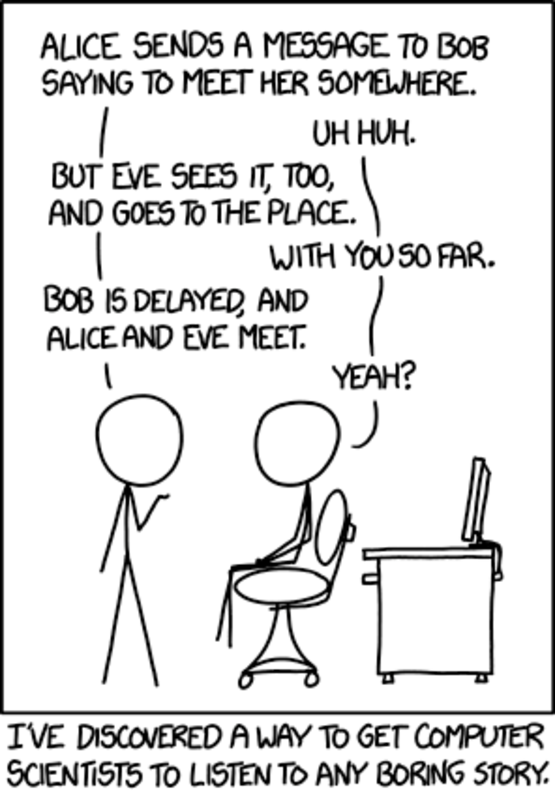
\includegraphics[width=45mm]{pic/alice-bob} 
\end{center}
\end{figure}
\end{frame}
\begin{frame}\frametitle{The Syntax of Encryption}
\begin{figure}
\begin{center}
\begin{tikzpicture}
\node (sender) [minimum size=1cm] {}; \Alice{0}{0}{0.4};
\node (bart) [below of = sender, node distance = 0.7cm] {Alice};
\node (enc) [draw, right of = sender, rounded corners=1ex,node distance = 2cm] {$\mathsf{Enc}$};
\node (k1) [above of = enc, node distance = 1cm] {$k$};
\node (c) [right of = enc, node distance = 2cm] {$c$};
\node (gen) [draw, above of = c, rounded corners=1ex,node distance = 1cm] {$\mathsf{Gen}$};
\node (adv) [below of = c, node distance = 1cm, minimum size=1cm] {}; \Evil{4cm}{-1cm}{0.4};
\node (burns) [below of = adv, node distance = 0.7cm] {Adversary};
\node (dec) [draw, right of = c, rounded corners=1ex,node distance = 2cm] {$\mathsf{Dec}$};
\node (k2) [above of = dec, node distance = 1cm] {$k$};
\node (receiver) [right of = dec, node distance = 2cm, minimum size=1cm] {}; \Bob{8cm}{0}{0.4};
\node (lisa) [below of = receiver, node distance = 0.7cm] {Bob};
\draw[-latex] (sender) -- (enc) node [midway, above] {$m$};
\draw (enc) -- (c); \draw[-latex] (c) -- (dec);
\draw[-latex] (dec) -- (receiver) node [midway, above] {$m$};
\draw[-latex] (k1) -- (enc);
\draw[-latex] (gen) -- (k1);
\draw[-latex] (gen) -- (k2);								
\draw[-latex] (k2) -- (dec);		
\end{tikzpicture}
\end{center}
\end{figure}
\begin{itemize}
\item key $k \in \mathcal{K}$, plaintext (or message) $m \in \mathcal{M}$, ciphertext $c \in \mathcal{C}$
\item \textbf{Key-generation} algorithm~$k \gets \mathsf{Gen}$
\item \textbf{Encryption} algorithm~$c:= \mathsf{Enc}_k(m)$
\item \textbf{Decryption} algorithm~$m:= \mathsf{Dec}_k(c)$
\item \textbf{Encryption scheme}: $\Pi = (\mathsf{Gen}, \mathsf{Enc}, \mathsf{Dec})$
\item \textbf{Basic correctness requirement}: $\mathsf{Dec}_k(\mathsf{Enc}_k(m)) = m$
\end{itemize}
\end{frame}
\begin{frame}\frametitle{Securing Key vs Obscuring Algorithm}
\begin{itemize}
\item Easier to maintain secrecy of a short key
\item In case the key is exposed, easier for the honest parties to change the key
\item In case many pairs of people, easier to use the same algorithm, but different keys
\end{itemize}
\begin{alertblock}{Kerckhoffs's principle}
\begin{quote}
The cipher method must not be required to be secret, and it must be able to fall into the hands of the enemy without inconvenience.
\end{quote}	
\end{alertblock}
\begin{alertblock}{Shannon's maxim}
	\begin{quote}
		The enemy knows the system.
	\end{quote}	
\end{alertblock}
\end{frame}
\begin{frame}\frametitle{Why ``Open Cryptographic Design''}
\begin{itemize}
\item Published designs undergo public scrutiny are to be stronger
\item Better for security flaws to be revealed by ``ethical hackers''
\item Reverse engineering of the code (or leakage by industrial espionage) poses a serious threat to security
\item Enable the establishment of standards.
\end{itemize}
\begin{exampleblock}{Dual EC: A Standardized Back Door}
	``Dual EC was standardized by NIST, ANSI, and ISO among other algorithms to generate pseudorandom numbers.'' ``The Snowden revelations, and in particular reports on Project Bullrun and the SIGINT Enabling Project, have indicated that Dual EC was part of a systematic effort by NSA to subvert standards.'' ``Reuters reported that NSA paid RSA ``\$10 million in a deal that set [Dual EC] as the preferred, or default, method for number generation in the BSafe software.''''	
\end{exampleblock}
\end{frame}
\begin{frame}\frametitle{Attack Scenarios}	
\begin{itemize}
\item \textbf{Ciphertext-only}: the adversary just observes ciphertext
\item \textbf{Known-plaintext}: the adversary learns pairs of plaintexts/ciphertexts under the same key
\item \textbf{Chosen-plaintext}: the adversary has the ability to obtain the encryption of plaintexts of its choice
\item \textbf{Chosen-ciphertext}: the adversary has the ability to obtain the decryption of \textbf{other} ciphertexts of its choice
\item \textbf{Passive attack}: COA KPA
\begin{itemize}
\item because not all ciphertext are confidential
\end{itemize}
\item \textbf{Active attack}: CPA CCA
\begin{itemize}
\item when to encrypt/decrypt whatever an adversary wishes?
\end{itemize}
\end{itemize}	
\end{frame}
\section{Historical Ciphers and Their Cryptanalysis}
\begin{comment}
	\begin{frame}\frametitle{Why We Learn Broken Ciphers?}
	\begin{itemize}
	\item To understand the weaknesses of an ``ad-hoc'' approach
	\item To learn that ``simple'' approaches are unlikely to succeed
	\item To feel that ``we are smart enough to do some crypt-analyzing''
	\end{itemize}
	\end{frame}
\end{comment}

\begin{frame}[fragile]\frametitle{Caesar's Cipher}
\begin{quote}
If he had anything confidential to say, he wrote it in cipher, that is, by so changing the order of the letters of the alphabet, that not a word could be made out. If anyone wishes to \alert{decipher} these, and get at their meaning, he must \alert{substitute the fourth letter of the alphabet, namely D, for A}, and so with the others

\rightline{--Suetonius,``Life of Julius Caesar''}
\end{quote}
\begin{itemize}
	\item $\mathsf{Enc}(m)=m+3\mod 26$ \footnote{In fact the quote indicates that decryption involved rotating letters of the alphabet forward 3 positions, $\mathsf{Dec}(c)=c+3\mod 26$}
	\item \textbf{Weakness}: ? %\alert{What is the key?}
\end{itemize}
\begin{exampleblock}{Example}
\verb|begintheattacknow|
%\verb|EHJLQWKHDWWDFNQRZ|
\end{exampleblock}
\end{frame}
\begin{frame}[fragile]\frametitle{Shift Cipher}
\begin{itemize}
\item $\mathsf{Enc}_k(m)=m+k\mod 26$
\item $\mathsf{Dec}_k(c)=c-k\mod 26$
\item \textbf{Weakness}: ? %Fragile under \textbf{Brute-force attack} (exhaustive search)
\end{itemize}
\begin{exampleblock}{Example: Decipher the string}	
\verb|EHJLQWKHDWWDFNQRZ|
\end{exampleblock}
\begin{alertblock}{Sufficient Key Space Principle}
Any secure encryption scheme must have a key space that is not vulnerable to exhaustive search.\footnote{If the plaintext space is larger than the key space.}
\end{alertblock}
\end{frame}
\begin{frame}\frametitle{Index of Coincidence (IC) Method (to find $k$)}
\textbf{How to automatically determine that the deciphered text makes sense?}

\textbf{Index of Coincidence (IC)}: the probability that two randomly selected letters (pick-then-return) will be identical.

Let $p_i$ denote the probability of $i$th letter in English text.
\[I \overset{\text{def}}{=}\sum_{i=0}^{25} p_i^2 \]
\begin{exampleblock}{Example}
What's the IC of `apple'?
\end{exampleblock}

For a long English text, the IC is $\approx 0.065$.
For $j = 0, 1, \dotsc , 25$, $q_j$ is the probability of $j$th letter in the ciphertext.
\[I_j \overset{\text{def}}{=}\sum_{i=0}^{25} p_i \cdot q_{i+j}\]
\alert{Q: For shift cipher, if $j = k$, then $I_j \approx$ ?}
\end{frame}

\begin{frame}[fragile]\frametitle{Mono-Alphabetic Substitution}
\begin{itemize}
\item \textbf{Idea}: To map each character to a different one in an arbitrary manner
\item \textbf{Strength}: Key space is large $\approx 2^{88}$. \alert{Q: how to count?}
\item \textbf{Weakness}: ? %The mapping of each letter is fixed
\end{itemize}
\begin{exampleblock}{Example}
\verb|abcdefghijklmnopqrstuvwxyz|\\
\verb|XEUADNBKVMROCQFSYHWGLZIJPT|

Plaintext: \verb|tellhimaboutme|\\
Ciphertext: \verb|??????????????|
\end{exampleblock}
\end{frame}
\begin{frame}[fragile]\frametitle{Attack with Statistical Patterns}
\begin{enumerate}
\item Tabulate the frequency of letters in the ciphertext
\item Compare it to those in English text
\item Guess the most frequent letter corresponds to \verb|e|, and so on
\item Choose the plaintext that does ``make sense'' (Not trivial)
\end{enumerate}
\begin{table}
\begin{center}
\caption{Average letter frequencies for English-language text}
\begin{tabular}{|cc|cc|cc|cc|cc|} \hline
e & 12.7\% & t & 9.1\% & a & 8.2\% & o & 7.5\% & i & 7.0\%\\
n & 6.7\% & \_ & 6.4\% & s & 6.3\% & h & 6.1\% & r & 6.0\%\\
d & 4.3\% & l & 4.0\% & c & 2.8\% & u & 2.8\% & m & 2.4\%\\
w & 2.4\% & f & 2.2\% & g & 2.0\% & y & 2.0\% & p & 1.9\%\\
b & 1.5\% & v & 1.0\% & k & 0.8\% & j & 0.2\% & x & 0.2\%\\
q & 0.1\% & z & 0.1\% & & & & & &\\ \hline
\end{tabular}
\end{center}
\end{table}
\end{frame}
\begin{frame}[fragile]\frametitle{Example of Frequency Analysis (Ciphertext)}
\begin{verbatim}
LIVITCSWPIYVEWHEVSRIQMXLEYVEOIEWHRXEXIPFEMVEWHKVS
TYLXZIXLIKIIXPIJVSZEYPERRGERIMWQLMGLMXQERIWGPSRIH
MXQEREKIETXMJTPRGEVEKEITREWHEXXLEXXMZITWAWSQWXSWE
XTVEPMRXRSJGSTVRIEYVIEXCVMUIMWERGMIWXMJMGCSMWXSJO
MIQXLIVIQIVIXQSVSTWHKPEGARCSXRWIEVSWIIBXVIZMXFSJX
LIKEGAEWHEPSWYSWIWIEVXLISXLIVXLIRGEPIRQIVIIBGIIHM
WYPFLEVHEWHYPSRRFQMXLEPPXLIECCIEVEWGISJKTVWMRLIHY
SPHXLIQIMYLXSJXLIMWRIGXQEROIVFVIZEVAEKPIEWHXEAMWY
EPPXLMWYRMWXSGSWRMHIVEXMSWMGSTPHLEVHPFKPEZINTCMXI
VJSVLMRSCMWMSWVIRCIGXMWYMX
\end{verbatim}
\end{frame}
\begin{frame}[fragile]\frametitle{Example of Frequency Analysis (Analysis)}
Count and Guess, Trial and Error.
\begin{table}
\begin{center}
\caption{Analysis Steps}
\begin{tabular}{|r|l|} \hline
Ciphertext & Plaintext \\ \hline
\alert{I}   & \alert{e} \\
\alert{XLI} & \alert{the} \\
\alert{E} & \alert{a} \\
\alert{R}tate & \alert{s}tate \\
atthatt\alert{MZ}e & atthatt\alert{im}e \\
he\alert{V}e & he\alert{r}e \\
remar\alert{A} & remar\alert{k} \\ \hline
\end{tabular}
\end{center}
\end{table}
\end{frame}
\begin{frame}[fragile]\frametitle{Example of Frequency Analysis (Plaintext)}
\begin{quote}
Hereupon Legrand arose, with a grave and stately air, and brought me the beetle
from a glass case in which it was enclosed. It was a beautiful scarabaeus, and, at
that time, unknown to naturalists -- of course a great prize in a scientific point
of view. There were two round black spots near one extremity of the back, and a
long one near the other. The scales were exceedingly hard and glossy, with all the
appearance of burnished gold. The weight of the insect was very remarkable, and,
taking all things into consideration, I could hardly blame Jupiter for his opinion
respecting it.

\rightline{--Edgar Allan Poe's ``The Gold-Bug''}
\end{quote}
\end{frame}

\begin{frame}[fragile]\frametitle{Vigen\`{e}re (poly-alphabetic shift) Cipher}
\begin{itemize}
\item \textbf{Idea}: To ``smooth out'' the distribution in the ciphertext by mapping different instances of the same letter in the plaintext to different ones in the ciphertext
\item \textbf{Encryption}: $c_i=m_i+k_{[i\bmod t]}$, $t$ is the length (period) of $k$
\item \textbf{Cryptanalysis}: Need find $t$; if $t$ is known, need know whether the decryption ``makes sense'', but brute force ($26^t$) is infeasible for $t > 15$
\end{itemize}
\begin{exampleblock}{Example (Key is `cafe')}
\begin{description}[Ciphertext]
\item[Plaintext]  \verb|tellhimaboutme| \\
\item[Key]        \verb|cafecafecafeca| \\
\item[Ciphertext] \verb|??????????????| %\verb|WFRQKJSFEPAYPF|
\end{description}
\end{exampleblock}
\end{frame}
\begin{frame}[fragile]\frametitle{Kasiski's Method (to find $t$)}
\begin{itemize}
\item To identify repeated patterns of length 2 or 3
\item The distance between such appearances is a multiple of $t$
\item $t$ is the greatest common divisor of all the distances
\end{itemize}
\begin{exampleblock}{Example (Key is `beads')}
\begin{semiverbatim}
themanandthewomanretrievedtheletterfromthepostoffice
beadsbeadsbeadsbeadsbeadsbeansdeadsbeadsbeadsbeadbea
VMFQTPFOH\alert{MJJ}XSFCSSIMTNFZXFYISEIYUIKHWPQ\alert{MJJ}QSLVTGJKGF
\end{semiverbatim}
\end{exampleblock}
\end{frame}
\begin{frame}\frametitle{Index of Coincidence (IC) Method (to find $t$)}
For $\tau = 1, 2, \dotsc$, $q_i$ is the probability of $i$th letter in $c_1, c_{1+\tau}, c_{1+2\tau}, \dotsc$, IC is
\[I_\tau \overset{\text{def}}{=}\sum_{i=0}^{25} q_i^2\]
\alert{If $\tau = t$, then $I_\tau \approx ?$} ; otherwise $q_i \approx \frac{1}{26}$ and
\[I_\tau \approx \sum_{i=0}^{25} \left(\frac{1}{26}\right)^2 \approx 0.038\]
Then reuse IC method to find $k_i$.
\begin{alertblock}{Arbitrary Adversary Principle}
Security must be guaranteed for any adversary within the class of adversaries having the specified power
\end{alertblock}
\end{frame}
\begin{frame}\frametitle{Cryptanalytic Attacks (homework assignment)}
\begin{itemize}
\item Under COA, the requirement for ciphertext related to the size of the key space.  Vig\`{e}nere > mono-alphabetic sub. > shift
\item Under KPA, trivially broken.
\end{itemize}
\begin{alertblock}{Lessons learned}
\begin{itemize}
\item Sufficient key space principle
\item Designing secure cipher is a hard task
\item Complexity does not imply security (then what does?)
\item Arbitrary adversary principle
\end{itemize}
\end{alertblock}
\end{frame}
\section{The Basic Principles of Modern Cryptography}
\begin{frame}\frametitle{Three Main Principles of Modern Cryptography}
\begin{enumerate}
\item The formulation of a rigorous \textbf{definition} of security / threat model
\item When the security of a cipher relies on an unproven \textbf{assumption}, this assumption must be precisely stated and be as minimal as possible
\item Cipher should be accompanied by a rigorous \textbf{proof} of security with the above definition and the above assumption
\end{enumerate}
\end{frame}
\begin{frame}\frametitle{Why Principle 1 -- Formulation of Exact Definitions}
\begin{exampleblock}{Q: how would you formalize the security for private-key encryption?}
\begin{enumerate}
\item \emph{No adversary can find the secret key when given a ciphertext.}\\
$\mathsf{Enc}_k(m)=m$
\item \emph{No adversary can find the plaintext that corresponds to the ciphertext.}\\
$\mathsf{Enc}_k(m)=m_{0}\| \mathsf{AES}_k(m)$
\item \emph{No adversary can determine any character of the plaintext that corresponds to the ciphertext.}\\
$m=1000$, someone can learn $ 800 < m < 1200$
\item \emph{No adversary can derive any meaningful information about the plaintext from the ciphertext.}\\
Could you define so-called `meaningful'?
\end{enumerate}
\emph{\alert{Definitions of security should suffice for all potential applications.}}
\end{exampleblock}
\end{frame}
\begin{frame}\frametitle{Why Principle 1 -- How to define}
%\begin{exampleblock}{General Form}
%A cryptographic scheme for a given \textbf{task} is secure if no adversary of a specified \textbf{power} can achieve a specified \textbf{break}
%\end{exampleblock}

How To Define Security -- Lesson From Alan Turing
\begin{itemize}
\item What's computation?\footnote{Q: Any ``mathematical proof that there exist well-defined problems that computers cannot solve''? A: Halting Problem in computability theory}
\begin{enumerate}
\item A direct appeal to \textbf{intuition}
\item A \textbf{proof of the equivalence} of two definitions\\ (The new one has a greater intuitive appeal)
\item Giving \textbf{examples} solved using a definition
\end{enumerate}
\item Additional method for security: \textbf{Test of time}
\end{itemize}
\end{frame}	
\begin{frame}\frametitle{Principle 2 -- Reliance on Precise Assumptions}
Most cryptographic constructions \textbf{cannot be proven secure unconditionally}
\begin{itemize}
	\item \textbf{Why?} 
	\begin{enumerate}
		\item Validation of the assumption
		\item Comparison of schemes
		\item Facilitation of proofs of security
	\end{enumerate}
	\textbf{The construction is secure if the assumption is true.}
	\item \textbf{How?} 
	\begin{enumerate}
		\item old, so well tested
		\item simple and lower-level, so easy to study, refute \& correct
	\end{enumerate}
\end{itemize}
\end{frame}
\begin{frame}\frametitle{Principle 3 -- Rigorous Proofs of Security}
\begin{itemize}
\item \textbf{Why?} Proofs are more desirable in computer security than in other fields.
\item \textbf{The reductionist approach}: 
\begin{theorem}	Given that Assumption X is true, Construction Y is secure according to the given definition.
\end{theorem}
\begin{proof} Reduce the problem given by X to the problem of breaking Y.
\end{proof}
\item \textbf{Ad-hoc approaches}: for those who need a ``quick and dirty'' solution, or who are just simply unaware.
\end{itemize}
\end{frame}
\begin{frame}\frametitle{Summary}
\begin{itemize}
\item Cryptography secures information, transactions and computations
\item Kerckhoffs's principle \& Open cryptographic design
\item Caesar's, shift, Mono-Alphabetic sub., Vigen\`{e}re
\item Brute force, letter frequency, Kasiski's, IC
\item Sufficient key space principle
\item Arbitrary adversary principle
\item Rigorously proven security
\end{itemize}
\end{frame}
\end{document}


%% presentation
\documentclass{beamer}
\usetheme[height=7mm]{Rochester}
\usecolortheme{rose}

% handout

%\documentclass[handout]{beamer}
%\usepackage{pgfpages} \pgfpagesuselayout{8 on 1}[a4paper]

%\documentclass[mathserif]{article}
%\usepackage{beamerarticle}

\usepackage{amsmath}
\usepackage{comment}
\usepackage{amssymb,amsfonts}
\usepackage[T1]{fontenc}
\usepackage{lmodern}
\usepackage{tikz}
%\usepackage{simpsons}
\usepackage{marvosym}
\usepackage{color}
\usepackage{multirow}
\usepackage{pgffor}
\usepackage{pgfplots}
\usepackage[slide,algoruled,titlenumbered,vlined,noend,linesnumbered,]{algorithm2e}

\usefonttheme{structurebold}

\setbeamertemplate{footline}[frame number]
\setbeamertemplate{navigation symbols}{}
\setbeamerfont{smallverb}{size*={73}}
\usefonttheme[onlymath]{serif}
\setbeamertemplate{theorems}[numbered]
\newtheorem{construction}[theorem]{Construction}
\newtheorem{proposition}[theorem]{Proposition}

\AtBeginSection[] {
  \begin{frame}
    \frametitle{Content}
    \tableofcontents[currentsection]
  \end{frame}
  \addtocounter{framenumber}{-1}
}

\usetikzlibrary[shapes.arrows]
\usetikzlibrary{shapes.geometric}
\usetikzlibrary{backgrounds}
\usetikzlibrary{positioning}
\usetikzlibrary{calc}
\usetikzlibrary{intersections}
\usetikzlibrary{fadings}
\usetikzlibrary{decorations.footprints}
\usetikzlibrary{patterns}
\usetikzlibrary{shapes.callouts}
\usetikzlibrary{fit}
%handout

\providecommand{\abs}[1]{\lvert#1\rvert}

\tikzset{every picture/.style={line width=1pt,show background rectangle},background rectangle/.style={fill=blue!10,rounded corners=2ex}}

\newcommand{\Bob}[3]{ \begin{scope}[shift={(#1,#2)},scale=#3]
  \draw (0,0) circle (0.95 and 1);
  \fill (-0.3,-0.1) circle (0.1);
  \fill (+0.3,-0.1) circle (0.1);
  \draw (0.35,-0.5) arc (-70:-110: 1 and 0.4);
  \draw (-0.3,0.5) arc (-10:-80: 0.8 and 0.8);
  \draw (-0.5,0.8) arc (190:255: 2 and 1);
  \draw (-0.7,0.9) -- +(0.2,-0.09) -- +(0.25,0.2);
  \end{scope} }

\newcommand{\Alice}[3]{ \begin{scope}[shift={(#1,#2)},scale=#3]
  \draw (0,0) circle (0.95 and 1);
  \fill (-0.3,-0.1) circle (0.1);
  \fill (+0.3,-0.1) circle (0.1);
  \draw (0.35,-0.5) arc (-70:-110: 1 and 0.4);
  \draw (0.3,1.3) arc (20:-100: 1.4 and 1);
  \draw (0.5,1.3) arc (150:260: 1 and 1);
  \draw (0.41,1.3) circle (0.35);
  \end{scope} }

  \newcommand{\Evil}[3]{ \begin{scope}[shift={(#1,#2)},scale=#3]
    \draw (0,0) circle (0.95 and 1);
    \fill (-0.1,-0.1) -- +(-0.2,-0.1) -- +(-0.4,0.2); %eye
    \fill (0.1,-0.1) -- +(0.2,-0.1) -- +(0.4,0.2);
    \draw (0.35,-0.5) arc (-70:-110: 1 and 0.4);
    %\fill (0.3,-0.5) -- +(-0.1,-0.2) -- +(-0.2,-0.02);
    %\fill (-0.3,-0.5) -- +(0.1,-0.2) -- +(0.2,-0.02);
    \fill (0.3,0.7) -- +(0.5,0.4) -- +(0.4,-0.2); % horn
    \fill (-0.3,0.7) -- +(-0.5,0.4) -- +(-0.4,-0.2);
    %\draw (0.3,1.3) arc (20:-100: 1.4 and 1);
    %\draw (0.5,1.3) arc (150:260: 1 and 1);
    %\draw (0.41,1.3) circle (0.35);
    \end{scope} }

\newcommand{\Charlie}[3]{ \begin{scope}[shift={(#1,#2)},scale=#3]
    \draw (0,0) circle (0.95 and 1);
    \filldraw[fill=black!20] (-0.35,-0.1) circle (0.25);
    \filldraw[fill=black!20] (+0.35,-0.1) circle (0.25);
    %\draw (0.9,0.2) to [bend left] (-0.9,0.2);
    \draw (0.2,0) to [bend left] (-0.2,0);


    %\draw (0.3,0.7) to [bend right] (-0.3,0.7);
    %\draw (0.4,0.5) to [bend right] (-0.4,0.5);
    %\draw (0.35,-0.5) arc (-70:-110: 1 and 0.4);
    \draw (-0.7,-0.6) to [bend right] (0,-0.6) to [bend right] (0.7,-0.6) to [bend right]  (0,-0.5)  to [bend right]  cycle ;
    %\draw (0.3,1.3) arc (20:-100: 1.4 and 1);
    %\draw (0.5,1.3) arc (150:260: 1 and 1);
    %\draw (0.41,1.3) circle (0.35);
    \end{scope} }

\author{Yu Zhang}
\institute{Harbin Institute of Technology}
\date[Crypto'22A]{Cryptography, Autumn, 2022}

%\input{1introduction.tex}
%\input{2perfectlysecret.tex}
%\input{3privatekey.tex}


\title{Perfectly Secret Encryption}

\begin{document}
\maketitle
\begin{frame}\frametitle{Outline}
\tableofcontents
\end{frame}
\section{Definitions and Basic Properties}
\begin{frame}\frametitle{Recall The Syntax of Encryption}
\begin{figure}
\begin{center}
\begin{tikzpicture}
\node (sender) [minimum size=1cm] {}; \Alice{0}{0}{0.4};
\node (bart) [below of = sender, node distance = 0.7cm] {Alice};
\node (enc) [draw, right of = sender, rounded corners=1ex,node distance = 2cm] {$\mathsf{Enc}$};
\node (k1) [above of = enc, node distance = 1cm] {$k$};
\node (c) [right of = enc, node distance = 2cm] {$c$};
\node (gen) [draw, above of = c, rounded corners=1ex,node distance = 1cm] {$\mathsf{Gen}$};
\node (adv) [below of = c, node distance = 1cm, minimum size=1cm] {}; \Evil{4cm}{-1cm}{0.4};
\node (burns) [below of = adv, node distance = 0.7cm] {Adversary};
\node (dec) [draw, right of = c, rounded corners=1ex,node distance = 2cm] {$\mathsf{Dec}$};
\node (k2) [above of = dec, node distance = 1cm] {$k$};
\node (receiver) [right of = dec, node distance = 2cm, minimum size=1cm] {}; \Bob{8cm}{0}{0.4};
\node (lisa) [below of = receiver, node distance = 0.7cm] {Bob};
\draw[-latex] (sender) -- (enc) node [midway, above] {$m$};
\draw (enc) -- (c); \draw[-latex] (c) -- (dec);
\draw[-latex] (dec) -- (receiver) node [midway, above] {$m$};
\draw[-latex] (k1) -- (enc);
\draw[-latex] (gen) -- (k1);
\draw[-latex] (gen) -- (k2);								
\draw[-latex] (k2) -- (dec);		
\end{tikzpicture}
\end{center}
\end{figure}
\begin{itemize}
\item $k \in \mathcal{K}, m \in \mathcal{M}, c \in \mathcal{C}$.
\item $k \gets \mathsf{Gen}, c:= \mathsf{Enc}_k(m), m:= \mathsf{Dec}_k(c)$.
\item \textbf{Encryption scheme}: $\Pi = (\mathsf{Gen}, \mathsf{Enc}, \mathsf{Dec})$.
\item \textbf{Random Variable}: $K, M, C$ for key, plaintext, ciphertext.
\item \textbf{Probability}: $\Pr[K=k], \Pr[M=m], \Pr[C=c].$
\item \alert{What's the basic correctness requirement?}
\end{itemize}
\end{frame}
\begin{frame}\frametitle{Definition of `Perfect Secrecy'}
\textbf{Intuition}: An adversary knows the probability distribution over $\mathcal{M}$. $c$ should have no effect on the knowledge of the adversary; the a \emph{posteriori} likelihood that some $m$ was sent should be no different from the a \emph{priori} probability that $m$ would be sent. 
\begin{definition}
$\Pi$ over $\mathcal{M}$ is \textbf{perfectly secret} if for every probability distribution over $\mathcal{M}$, $\forall m \in \mathcal{M}$ and $\forall c \in \mathcal{C}$ for which $\Pr[C = c] > 0$:
\[ \Pr[M=m | C=c] = \Pr[M=m].\]
\end{definition}
\textbf{Simplify}: non-zero probabilities for $\forall m \in \mathcal{M}$ and $\forall c \in \mathcal{C}$.\\

\begin{exampleblock}{Is the below scheme perfectly secret?}{ For $\mathcal{M}=\mathcal{K} = \{ 0,1 \} , \mathsf{Enc}_k(m)= m \oplus k$.}\end{exampleblock}
\end{frame}

\begin{frame}\frametitle{Perfect Secrecy On One Bit}

\begin{exampleblock}{XORing one bit is perfectly secret.}
Let $\Pr[M=1] = p$ and $\Pr[M=0] = 1-p$.
Let us consider a case that $M=1$ and $C=1$.
\[ \Pr[M=1 | C=1] = \Pr[C=1 | M=1 ] \cdot \Pr[ M=1 ] / \Pr[C=1] \]
\[ = \frac{\Pr[K = 1\oplus 1] \cdot p }{ \Pr[C=1 | M=1] \cdot \Pr[M=1] + \Pr[C=1 | M=0] \cdot \Pr[M=0]} \]
\[ = \frac{1/2 \cdot p }{ 1/2 \cdot p + 1/2 \cdot (1-p)} = p = \Pr[M=1] \]
We can do the same for other cases.
\end{exampleblock}
Note that $\Pr[M=1 | C=1] \neq \Pr[M=1, C=1] = \Pr[C=1 | M=1] \cdot \Pr[M=1] = 1/2 \cdot p$.
\end{frame}

\begin{frame}\frametitle{An Equivalent Formulation}
\begin{lemma} \label{lem:ps} 
$\Pi$ over $\mathcal{M}$ is perfectly secret $\iff$ for every probability distribution over $\mathcal{M}$, $\forall m \in \mathcal{M}$ and $\forall c \in \mathcal{C}$:
\[ \Pr[C=c | M=m] = \Pr[C=c].\]
\end{lemma}
\begin{proof}
$\Leftarrow$: Multiplying both sides by $\Pr[M=m]/\Pr[C=c]$, then use Bayes' Theorem.\footnote{If $\Pr[B]\neq 0$ then $ \Pr[A|B] = \left( \Pr[A] \cdot \Pr[B|A] \right) / \Pr[B] $} \\
$ \Pr[C=c | M=m] \cdot \Pr[M=m] / \Pr[C=c] = \Pr[M=m]$\\
$ \Pr[M=m | C=c] \cdot \Pr[C=c] / \Pr[C=c] = \Pr[M=m | C=c]$
$\Rightarrow$: Multiplying both sides by $\Pr[C=c]/\Pr[M=m]$, then use Bayes' Theorem.
\end{proof}
\end{frame}
\begin{frame}\frametitle{Perfect Indistinguishability}
\begin{lemma}\label{lem:pi}
$\Pi$ over $\mathcal{M}$ is perfectly secret $\iff$ for every probability distribution over $\mathcal{M}$, $\forall m_0, m_1 \in \mathcal{M}$ and $\forall c \in \mathcal{C}$:
\[ \Pr[C=c | M=m_0] = \Pr[C=c | M=m_1].\]
\end{lemma}
\begin{proof}
$\Rightarrow$: By Lemma \ref{lem:ps}: $\Pr[C=c | M=m] = \Pr[C=c]$. \\
$\Leftarrow$: $p \overset{\text{def}}{=} \Pr[C=c | M=m_0]$.
\[
\begin{split}
	\Pr[C=c] &= \sum_{m \in \mathcal{M}} \Pr[C=c|M=m] \cdot \Pr[M=m] \\
	&= \sum_{m \in \mathcal{M}} p \cdot \Pr[M=m] = p = \Pr[C=c|M=m_0].
\end{split}
\]
\end{proof}
\end{frame}
\section{The One-Time Pad (Vernam's Cipher)}
\begin{frame}\frametitle{One-Time Pad (Vernam's Cipher)}
\begin{itemize}
	\item $\mathcal{M} = \mathcal{K} = \mathcal{C} = \{0,1\}^{\ell}$.
	\item $\mathsf{Gen}$ chooses a $k$ randomly with probability exactly $2^{-\ell}$.
	\item $c := \mathsf{Enc}_k(m) = k \oplus m$. 
	\item $m := \mathsf{Dec}_k(c) = k \oplus c$. 
\end{itemize}
\begin{theorem}
The one-time pad encryption scheme is perfectly-secret.
\end{theorem}
\begin{proof}
\[\begin{split} \Pr[C=c|M=m] &= \Pr[M \oplus K=c|M=m] \\
&= \Pr[m \oplus K=c] = \Pr[K = m \oplus c] = 2^{-\ell}.
\end{split}
\]
Then Lemma \ref{lem:pi}: $\Pr[C=c | M=m_0] = \Pr[C=c | M=m_1]$.
\end{proof}
\end{frame}
\section{Limitations of Perfect Secrecy}
\begin{frame}\frametitle{Limitations of OTP and Perfect Secrecy}
Key $k$ is as long as $m$, difficult to store and share $k$.
\begin{theorem}
Let $\Pi$ be perfectly-secret over $\mathcal{M}$, and let $\mathcal{K}$ be determined by $\mathsf{Gen}$. Then $|\mathcal{K}|\ge |\mathcal{M}|$. 
\end{theorem}
\begin{proof}
Assume $|\mathcal{K}| < |\mathcal{M}|$.
$\mathcal{M}(c) \overset{\text{def}}{=} \{ \hat{m} | \hat{m} = \mathsf{Dec}_k(c)\  \text{for some}\ \hat{k} \in \mathcal{K} \}$. Since for one $k$, there is at most one $m$ such that $m = \mathsf{Dec}_k(c)$, $|\mathcal{M}(c)|\le |\mathcal{K}| < |\mathcal{M}|$. So $\exists m' \notin \mathcal{M}(c)$. Then
\[ \Pr[M=m'|C=c] = 0 \neq \Pr[M = m'] \]
and so not perfectly secret.
\end{proof}
\end{frame}
\begin{frame}\frametitle{Two Time Pad: Real World Cases}
Only used once for the same key, otherwise
\[c\oplus c'=(m\oplus k)\oplus (m'\oplus k)=m\oplus m'.\]
Learn $m$ from $m\oplus m'$ due to the redundancy of language.
\begin{exampleblock}{MS-PPTP (Win NT)}
\begin{figure}
\begin{center}
\begin{tikzpicture}
\node (sender) [minimum size=1cm,label=below:Client, label=above:$k$] {}; \Alice{0}{0}{0.4};
\node (c) at ($(sender)+(4cm,0.5cm)$) {$\left[ m_1\|m_2\|m_3\right] \oplus PRG(k)$};
\node (c1) [below of = c, node distance = 1cm] {$\left[s_1\|s_2\|s_3\right] \oplus PRG(k)$};
\node (receiver) at ($(sender)+(8cm,0)$) [minimum size=1cm,label=below:Server, label=above:$k$] {}; \Bob{8cm}{0}{0.4};
\draw[-latex] (sender.east |- c) -- (c) -- (receiver.west |- c);
\draw[-latex] (receiver.west |- c1) -- (c1) -- (sender.east |- c1);
\end{tikzpicture}
\end{center}
\end{figure}
Improvement: use two keys for C-to-S and S-to-C separately.
\end{exampleblock}
\end{frame}
\section{Shannon's Theorem}
\begin{frame}\frametitle{Shannon's Theorem}
\begin{theorem}
For $|\mathcal{M}| = |\mathcal{K}| = |\mathcal{C}|$, $\Pi$ is perfectly secret $\iff$
\begin{enumerate}
\item Every $k \in \mathcal{K}$ is chosen with probability $1/|\mathcal{K}|$ by $\mathsf{Gen}$.
\item $\forall m \in \mathcal{M}$ and $\forall c \in \mathcal{C}$, $\exists$ unique $k \in \mathcal{K}$: $c := \mathsf{Enc}_k(m)$.
\end{enumerate}
\end{theorem}
\begin{proof}
$\Leftarrow$: $\Pr[C=c|M=m]=1/|\mathcal{K}|$, use Lemma \ref{lem:pi}. \\
$\Rightarrow (2)$: At least one $k$, otherwise $\Pr[C=c|M=m]=0$; \\
at most one $k$, because $\{\mathsf{Enc}_k(m)\}_{k\in \mathcal{K}} = \mathcal{C}$ and $|\mathcal{K}| = |\mathcal{C}|$.\\
$\Rightarrow (1)$: $k_i$ is such that $\mathsf{Enc}_{k_i}(m_i)=c$.
\[ \begin{split}
\Pr[M = m_i] &= \Pr[M=m_i|C=c] \\
             &= \left( \Pr[C =c|M=m_i] \cdot \Pr[M = m_i] \right) / \Pr[C=c] \\
 &= \left( \Pr[K=k_i] \cdot \Pr[M = m_i] \right) / \Pr[C=c],
\end{split}
\]
so $\Pr[K=k_i] = \Pr[C = c] = 1/|\mathcal{K}|$.
\end{proof}
\end{frame}

\begin{frame}\frametitle{Application of Shannon's Theorem}
\begin{exampleblock}{Is the below scheme perfectly secret?}
Let $\mathcal{M} = \mathcal{C} = \mathcal{K} = \{ 0, 1, 2,\dots , 255 \} $\\
$\mathsf{Enc}_k(m) = m  + k \mod 256$\\
$\mathsf{Dec}_k(c) = c - k \mod 256$
\end{exampleblock}
\end{frame}
\section{Eavesdropping Indistinguishability}
\begin{frame}\frametitle{Eavesdropping Indistinguishability Experiment}
$\mathsf{PrivK}^{\mathsf{eav}}_{\mathcal{A},\Pi}$ denote a \textbf{priv}ate-\textbf{k}ey encryption experiment for a given $\Pi$ over $\mathcal{M}$ and an \textbf{eav}esdropping adversary $\mathcal{A}$.
\begin{enumerate}
	\item $\mathcal{A}$ outputs a pair of messages $m_0, m_1 \in \mathcal{M}$.
	\item $k \gets \mathsf{Gen}$, a random bit $b \gets \{0,1\}$ is chosen. Then $c \gets \mathsf{Enc}_k(m_b)$ is given to $\mathcal{A}$.
	\item $\mathcal{A}$ outputs a bit $b'$
	\item If $b' = b$, $\mathcal{A}$ succeeded $\mathsf{PrivK}^{\mathsf{eav}}_{\mathcal{A},\Pi}=1$, otherwise 0.
\end{enumerate}
\begin{figure}
\begin{center}
\begin{tikzpicture}
%\node (A) at (0,0) {\Homer};
%\node (B) [right of = A, node distance = 4cm] {\Left\Burns};
\node (A) at (0,0) [minimum size=1cm] {}; \Charlie{0}{0}{0.4};
\node (B) [right of = A, node distance = 4cm, minimum size=1cm] {}; \Evil{4cm}{0}{0.4};
\node (1a) [below of=A, node distance=1cm] {};
\node (1b) [below of=B, node distance=1cm] {$m_0, m_1$};
\draw[-latex] (1b) -- (1a) node [midway,above] {};
\node (2a) [below of=1a, node distance=0.5cm] {Gen $b, k$};
\node (2b) [below of=1b, node distance=0.5cm] {};
%\draw[-latex] (2b) -- (2a) node [midway,above] {};
%\node (3a) [below of=2a, node distance=0.5cm] {};
%\node (3b) [below of=2b, node distance=0.5cm] {};
\node (4a) [below of=2a, node distance=0.5cm] {$\mathsf{Enc}_k(m_b)$};
\node (4b) [below of=2b, node distance=0.5cm] {};
\draw[-latex] (4a) -- (4b) node [midway,above] {};
\node (5a) [below of=4a, node distance=0.5cm] {};
\node (5b) [below of=4b, node distance=0.5cm] {$b'$};
\draw[-latex] (5b) -- (5a) node [midway,above] {};
\node (6a) [below of=5a, node distance=0.5cm] {};
\node (6b) [below of=5b, node distance=0.5cm] {};
\node (result) [right of = 6a, node distance = 2cm] {Win if $b = b'$};
\end{tikzpicture}

\end{center}
\end{figure}
\end{frame}
\begin{frame}\frametitle{Adversarial Indistinguishability}
\begin{definition}
$\Pi$ over $\mathcal{M}$ is \textbf{perfectly secret} if for every $\mathcal{A}$ it holds that
\[ \Pr[\mathsf{PrivK}^{\mathsf{eav}}_{\mathcal{A},\Pi}=1] = \frac{1}{2}.\]
\end{definition}
\begin{exampleblock}{Which in the below schemes are perfectly secret?}
\begin{itemize}
\item $\mathsf{Enc}_{k,k'}(m)= \mathsf{OTP}_k(m) \| \mathsf{OTP}_{k'}(m)$
\item $\mathsf{Enc}_{k}(m)= reverse(\mathsf{OTP}_k(m))$
\item $\mathsf{Enc}_{k}(m)= \mathsf{OTP}_k(m) \| k$
%To break semantic security, an attacker would read the secret key from the challenge ciphertext and use it to decrypt the challenge ciphertext. Basically, any ciphertext reveals the secret key.
\item $\mathsf{Enc}_{k}(m)= \mathsf{OTP}_k(m) \| \mathsf{OTP}_k(m) $
\item $\mathsf{Enc}_{k}(m)= \mathsf{OTP}_{0^{n}}(m)$
%To break semantic security, an attacker would ask for the encryption of $0^n$ and $1^n$ and can easily distinguish EXP(0) from EXP(1) because it knows the secret key, namely 0n.
\item $\mathsf{Enc}_{k}(m)= \mathsf{OTP}_k(m) \| LSB(m)$
%To break semantic security, an attacker would ask for the encryption of $0^n$ and $0^{n-1}1$ and can distinguish EXP(0) from EXP(1).
\end{itemize}
\end{exampleblock}
\end{frame}

\begin{frame}\frametitle{Summary}
\begin{itemize}
\item Perfect secrecy $=$ Perfect indistinguishability $=$ Adversarial indistinguishability
\item Perfect secrecy is attainable. The One-Time Pad (Vernam's cipher)
\item Shannon's theorem
\end{itemize}	
\end{frame}
\end{document}

%\input{3privatekey.tex}


\title{RSA Problem and Encryption}

\begin{document}
\maketitle
\begin{frame}
\frametitle{Outline}
\tableofcontents
\end{frame}
\section{RSA Problem}
\begin{frame}\frametitle{RSA Overview}
\begin{itemize}
\item \textbf{RSA}: Ron Rivest, Adi Shamir and Leonard Adleman, in 1977
\item \textbf{RSA problem}: Given $N = pq$ (two distinct big prime numbers) and $y \in \mathbb{Z}^*_N$, compute $y^{-e}$, $e^{\text{th}}$-root of $y$ modulo $N$
\item \alert{Open problem}:RSA problem is easier than factoring $N$?
\item \textbf{Standards}: PKCS\#1 (RFC3447/8017), ANSI X9.31, IEEE 1363
\item \textbf{Key sizes}: 1,024 to 4,096 bit
\item \textbf{Best public cryptanalysis}: a 768 bit key has been broken
\item \textbf{RSA Challenge}: break RSA-2048 to win \$200,000 USD
\end{itemize}
\textbf{Key lengths} with comparable security :
\begin{center}
\begin{tabular}{|c|c|} \hline
Symmetric & RSA  \\ \hline
80 bits & 1024 bits   \\
128 bits & 3072 bits  \\
256 bits & 15360 bits \\ \hline
\end{tabular}	
\end{center}
\end{frame}
\begin{frame}\frametitle{``Textbook RSA''}
\begin{construction}
\begin{itemize}
\item $\mathsf{Gen}$: on input $1^n$ run $\mathsf{GenRSA}(1^n)$ to obtain $N,e,d$. $pk = \langle N,e \rangle$ and $sk = \langle N,d \rangle$.
\item $\mathsf{Enc}$: on input $pk$ and $m \in \mathbb{Z}^*_N$, $c:= [m^e \bmod N]$.
\item $\mathsf{Dec}$: on input $sk$ and $m \in \mathbb{Z}^*_N$, $m:= [c^d \bmod N]$.
\end{itemize}
\end{construction}
\begin{alertblock}{Insecurity}
Since the ``textbook RSA'' is deterministic, it is insecure with respect to any of the definitions of security we have proposed. 
\end{alertblock}
\alert{Q: How to generate $N,e,d$? What's $\mathbb{Z}^*_N$? How to compute $m^e \bmod N$? Is it TDP? Why is it hard?}
\begin{block}{Textbook}
``\emph{A Computational Introduction to Number Theory and Algebra}''
(Version 2) by Victor Shoup
\end{block}
\end{frame}
\begin{frame}\frametitle{Primes and Modular Arithmetic}
\begin{itemize}
\item The set of \textbf{integers} $\mathbb{Z}$, $a,b,c \in \mathbb{Z}$.
%\item $a$ \textbf{divides} $b$: $a \mid b$ if $\exists c, ac=b$ (otherwise $a \nmid b$). \\$b$ is a \textbf{multiple} of $a$. If $a \notin \{1,b\}$, then $a$ is a \textbf{factor} of $b$. 
\item $p > 1$ is \textbf{prime} if it has no factors; otherwise, \textbf{composite}.
%\item $\forall a,b$, $\exists$ \textbf{quotient} $q$, \textbf{remainder} $r$: $a=qb+r$, and $0\le r < b$.
\item \textbf{Greatest common divisor} $\gcd(a,b)$ is the largest integer $c$ such that $c\mid a$ and $c\mid b$. $\gcd(0,b)=b$, $\gcd(0,0)$ undefined.
%\item $a$ and $b$ are \textbf{relatively prime (coprime)} if $\gcd(a,b)=1$.
%\item \textbf{Euclid's theorem}: there are infinitely many prime numbers.
\item Remainder $r= [a\bmod N] = a - b\lfloor a/b\rfloor $  and $r<N$. $N$ is called \textbf{modulus}.
\item $\mathbb{Z}_N = \{0,1,\dots,N-1\} = \{a \bmod N | a \in \mathbb{Z}\}$.
\item $a$ is \textbf{invertible modulo} $N$ $\iff \gcd(a,N) = 1$. If $ab \equiv 1 \pmod N$, then $b=a^{-1}$ is \textbf{multiple inverse} of $a$ \textbf{modulo} $N$.
\end{itemize}
\end{frame}
%\begin{frame}\frametitle{Fundamental Theorem of Arithmetic}
%\begin{itemize}
%\item \textbf{B\'{e}zout's lemma}: $\forall a,b,\;\exists\;X,Y:\;Xa+Yb=\gcd(a,b)$. $\gcd(a,b)$ is the smallest positive integer that can be expressed in this way.
%\item \textbf{Euclid's lemma}: If $c \mid ab$ and $\gcd(a,c)=1$, then $c \mid b$. \\
%If $p$ is prime and $p\mid ab$, then either $p \mid a$ or $p \mid b$.
%\item \textbf{Fundamental theorem of arithmetic}: $\forall N >1$, $N = \prod _i p_i^{e_i}$, $\{p_i\}$ are distinct primes and $e_i \ge 1$. This expression is unique.
%\end{itemize}
%\end{frame}
%\begin{frame}\frametitle{Modular Arithmetic}
%\begin{itemize}
%\item Remainder $r= [a\bmod N] = a - b\lfloor a/b\rfloor $  and $r<N$. $N$ is called \textbf{modulus}.
%%\item \textbf{Reduction modulo} $N$: mapping $a$ to $[a \bmod N]$.
%\item $\mathbb{Z}_N = \{0,1,\dots,N-1\} = \{a \bmod N | a \in \mathbb{Z}\}$.
%\item $a$ and $b$ are \textbf{congruent modulo} $N$: $a \equiv b \pmod N$ if $[a \bmod N] = [b \bmod N]$.
%\item $a$ is \textbf{invertible modulo} $N$ $\iff \gcd(a,N) = 1$. If $ab \equiv 1 \pmod N$, then $b=a^{-1}$ is \textbf{multiple inverse} of $a$ \textbf{modulo} $N$.
%\item \textbf{Cancellation law}: If $\gcd(a,N)=1$ and $ab \equiv ac \pmod N$, then $b \equiv c \pmod N$.
%\item \textbf{Euclidean algorithm}: $\gcd(a,b) = \gcd(b, [a \bmod b]).$
%\item \textbf{Extended Euclidean algorithm}: Given $a,N$, find $X,Y$ with $Xa+YN = \gcd(a,N)$.
%\end{itemize}
%\end{frame}
\begin{frame}\frametitle{Examples of Modular Arithmetic}
\textbf{Euclidean algorithm}: $\gcd(a,b) = \gcd(b, [a \bmod b]).$
\begin{exampleblock}{Find $\gcd(12, 27)$}
%$(-3)\cdot 11 + 2\cdot 17 = 1$, so 14 is the inverse of 11.
\end{exampleblock}
\textbf{Extended Euclidean algorithm}: Given $a,N$, find $X,Y$ with $Xa+YN = \gcd(a,N)$\footnote{B\'{e}zout's lemma}.
\begin{exampleblock}{Find the inverse of $11 \pmod {17}$}
%$(-3)\cdot 11 + 2\cdot 17 = 1$, so 14 is the inverse of 11.
\end{exampleblock}
Reduce and then add/multiply
\begin{exampleblock}{Compute $193028 \cdot 190301 \bmod 100$}
%[193028 \bmod 100] \cdot [190301 \bmod 100] \bmod 100 = ?$
%$= 28\cdot 1 \equiv 28 \bmod 100.$
\end{exampleblock}
\textbf{Cancellation law}: If $\gcd(a,N)=1$ and $ab \equiv ac \pmod N$, then $b \equiv c \pmod N$.
\begin{exampleblock}{$a=3, c=10, b=2, N=24$}
%$3\cdot 2 = 6 \equiv 3 \cdot 10 \pmod{24}$, but $2 \not \equiv 10 \pmod{24}$.
\end{exampleblock}
\end{frame}
\begin{frame}\frametitle{$\mathbb{Z}_N^*$ Group}
\[ \mathbb{Z}_N^* \overset{\text{def}}{=} \{a \in \{1,\dotsc,N-1 \} | \gcd(a,N) = 1\} \]
A \textbf{group} is a set $\mathbb{G}$ with a binary operation $\circ$:
\begin{itemize}
\item (\textbf{Closure}:) $\forall g,h \in \mathbb{G}$, $g \circ h \in \mathbb{G}$.
\item (\textbf{Existence of an Identity}:) $\exists$ \textbf{identity} $e\in \mathbb{G}$ such that $\forall g\in \mathbb{G}, e \circ g = g = g \circ e$.
\item (\textbf{Existence of Inverses}:) $\forall g \in G$, $\exists\; h \in \mathbb{G}$ such that $g \circ h =e = h \circ g$. $h$ is an \textbf{inverse} of $g$.
\item (\textbf{Associativity}:) $\forall g_1,g_2,g_3 \in \mathbb{G}$, $(g_1\circ g_2)\circ g_3 = g_1 \circ (g_2 \circ g_3)$.
\end{itemize}
$\mathbb{G}$ with $\circ$ is \textbf{abelian} if
\begin{itemize}
\item (\textbf{Commutativity}:) $\forall g,h \in \mathbb{G}, g\circ h = h\circ g$.
\end{itemize}
Existence of inverses implies \textbf{cancellation law}.\\
When $\mathbb{G}$ is a \textbf{finite group} and $\abs{\mathbb{G}}$ is the \textbf{order} of group.
\begin{exampleblock}{
$\mathbb{Z}_{15}^* = ?$ $\mathbb{Z}_{13}^* = ?$ Is $\mathbb{Z}_N^*$ a group under `$\cdot$'?}
\end{exampleblock}
\end{frame}
\begin{frame}\frametitle{Group Exponentiation}
%\[mg = m\cdot g \overset{\text{def}}{=} \underbrace{g+\cdots +g}_{m\; \text{times}}.\]
\[ g^m \overset{\text{def}}{=} \underbrace{g\circ g\circ \cdots \circ g}_{m\; \text{times}}. \]
\begin{theorem}
Euler's theorem: $\mathbb{G}$ is a finite group. Then $\forall g \in \mathbb{G}, g^{\abs{\mathbb{G}}}=1$.
\end{theorem}
\begin{exampleblock}{Calculate all exponentiation of $3 \in \mathbb{Z}_{7}^*$}
\end{exampleblock}
\begin{corollary}
Fermat's little theorem: $\forall g \in \mathbb{G}$ and $i$, $g^i \equiv g^{[i \bmod {\abs{\mathbb{G}}}]}$.
\end{corollary}
\begin{exampleblock}{Calculate $3^{78} \in \mathbb{Z}_{7}^*$}
\end{exampleblock}
%\begin{corollary}
%Define function $f_e\;:$ $\mathbb{G} \to \mathbb{G}$ by $f_e(g) =g^e$. \\
%If $\gcd(e,\abs{\mathbb{G}})=1$, then $f_e$ is a permutation. \\
%Let $d = [e^{-1} \bmod {\abs{\mathbb{G}}}]$, then $f_d$ is the inverse of $f_e$. ($f_d(f_e(g))=g$)\\
%\textbf{$e$'th root of $c$}: $g^e = c$, $g = c^{1/e} = c^{d}$. 
%\end{corollary}
\end{frame}
\begin{frame}\frametitle{Arithmetic algorithms}
\begin{itemize}
\item \textbf{Addition/subtraction}: linear time $O(n)$.
\item \textbf{Mulplication}: naively $O(n^2)$. Karatsuba (1960): $O(n^{\log_2 3})$\\
Basic idea: $(2^bx_1+x_0) \times (2^by_1+ y_0)$ with 3 mults.\\
Best (asymptotic) algorithm: about $O(n\log n)$.
\item \textbf{Division with remainder}: $O(n^2)$.
\item \textbf{Exponentiation}: $O(n^3)$.
\end{itemize}
\begin{algorithm}[H]
\SetKwInOut{Input}{input}
\SetKwInOut{Output}{output}
\SetKw{KwB}{break}
\SetKw{KwH}{halt}
\DontPrintSemicolon
\caption{Exponentiating by Squaring}
\Input{$g \in G$; exponent $x=[x_nx_{n-1}\dots x_2x_1x_0]_2$}
\Output{$g^x$}
\BlankLine
$y \gets g; z \gets 1$\;
\For{$i = 0$ \KwTo $n$}{
  \lIf{$x_i == 1$}{$z \gets z \times y$}
  $y \gets y^2$\;
}
\Return $z$
\end{algorithm}
\end{frame}
\begin{frame}\frametitle{Euler's Phi Function}
%\[ \mathbb{Z}_N^* \overset{\text{def}}{=} \{a \in \{1,\dotsc,N-1 \} | \gcd(a,N) = 1\} \]
\textbf{Euler's phi function}: $\phi(N) \overset{\text{def}}{=} \abs{\mathbb{Z}_N^*}$.
\begin{theorem}
$N = \prod_ip_i^{e_i}$ \footnote{Fundamental theorem of arithmetic}, $\{p_i\}$ are distinct primes, $\phi(N) = \prod_ip_i^{e_i-1}(p_i-1)$.
\end{theorem}
\begin{exampleblock}{$N=pq$ where $p,q$ are distinct primes. $\phi(N)=?$ $\phi(12)=?\quad \phi(30)=?$}
\end{exampleblock}
\begin{corollary}[Euler's theorem \& Fermat's little theorem]
$a \in \mathbb{Z}_N^*$. $a^{\phi (N)} \equiv 1 \pmod N$.\\
If $p$ is prime and $a \in \{1,\dotsc,p-1\}$, then $a^{p-1} \equiv 1 \pmod p$.
\end{corollary}
\begin{exampleblock}{$3^{43} \bmod 49 = ?$}
\end{exampleblock}
\end{frame}
\begin{frame}\frametitle{Permutation by Group Exponentiation Function}
\textbf{Exponentiation function} $f_e\;:$ $\mathbb{Z}^*_N \to \mathbb{Z}^*_N$ by $f_e(x) =[x^e \bmod N]$.\\
\textbf{$e$'th root of $y$}: $x^e \equiv y$, $x \equiv y^{1/e}$. 
\begin{corollary}
If $\gcd(e,\phi(N))=1$, then $f_e$ is a permutation.
\end{corollary}
\begin{proof}
Let $d = [e^{-1} \bmod \phi(N)]$, then $f_d$ is the inverse of $f_e$.\\
$y \equiv x^{e};\quad f_{d}(y) \equiv y^d \equiv x^{ed} \equiv x$. 
\end{proof}
\begin{exampleblock}{In $\mathbb{Z}^*_{10}$,\ $e = 3,\ d = ?,\ f_{e}(3) = ?,\ f_{d}(f_{e}(3)) = ?,\ 9^{\frac{1}{3}} = ?$}
\end{exampleblock}
\begin{alertblock}{What if we cannot get $\phi(N)$ for some `special' $N$?\\
What if we cannot factorize these `special' $N$?}
\end{alertblock}
\end{frame}
\begin{frame}\frametitle{Factoring Is Hard}
\begin{itemize}
\item \textbf{Factoring} $N=pq$. $p,q$ are of the same length $n$.
\item \textbf{Trial division}: $\mathcal{O}(\sqrt{N}\cdot \mathsf{polylog}(N))$.
\item \textbf{Pollard's $p-1$} method: effective when $p-1$ has ``small'' prime factors.
\item \textbf{Pollard's rho} method: $\mathcal{O}(N^{1/4}\cdot \mathsf{polylog}(N))$.
\item \textbf{Quadratic sieve} algorithm [Carl Pomerance]: sub-exponential time $\mathcal{O}(\exp(\sqrt{n\cdot \log n}))$.
\item The best-known algorithm is the \textbf{general number field sieve} [Pollard] with time $\mathcal{O}(\exp(n^{1/3}\cdot(\log n)^{2/3}))$.
\end{itemize}
\end{frame}
\begin{frame}\frametitle{The RSA Problem Is Hard}
\textbf{Idea}: factoring is hard\\ $\implies$ for $N=pq$, finding $p,q$ is hard\\ $\implies$ computing $\phi(N)=(p-1)(q-1)$ is hard\\ 
%$\implies$ computations modulo $\phi(N)$ is not available\\ 
$\implies$ computing $e^{-1} \bmod \phi(N)$ is hard\\
\alert{\textbf{There is a gap.}}\\
$\implies$ RSA problem is hard:\\
Given $y \in \mathbb{Z}^*_N$, compute $y^{-e}$ modulo $N$.
\begin{alertblock}{Open problem}
RSA problem is easier than factoring?
\end{alertblock}
\end{frame}
\begin{comment}
\begin{frame}\frametitle{Subgroups}
If $\mathbb{G}$ is a group, a set $\mathbb{H} \subseteq \mathbb{G}$ is a \textbf{subgroup} of $\mathbb{G}$ if $\mathbb{H}$ itself forms a group under the same operation associated with $\mathbb{G}$. $\mathbb{H}$ is a \textbf{strict subgroup} if $\mathbb{H} \neq \mathbb{G}$.
\begin{itemize}
\item If $\mathbb{H} \subseteq \mathbb{G}$, $\mathbb{H}$ contains the identity element of $\mathbb{G}$, and $\mathbb{H}$ is closed, then $\mathbb{H}$ is a subgroup of $\mathbb{G}$.
\item \textbf{Lagrange's theorem}: For a finite group $\mathbb{G}$ and its subgroup $\mathbb{H}$,  $\abs{\mathbb{H}} \mid \abs{\mathbb{G}}$.
\item $\mathbb{H}$ is a strict subgroup of a finite group $\mathbb{G}$, then $\abs{\mathbb{H}} \le \abs{\mathbb{G}}/2$.
\end{itemize}
\end{frame}
\begin{frame}\frametitle{Examples on Groups}
\begin{exampleblock}{}
\begin{itemize}
\item $\mathbb{Z}$ is an abelian group under `$+$', not a group under `$\cdot$'.
\item The set of real numbers $\mathbb{R}$ is not a group under `$\cdot$'.
\item $\mathbb{R}\setminus \{0\}$ is an abelian group under `$\cdot$'.
\item $\mathbb{Z}_N$ is an abelian group under `$+$' modulo $N$.
\item If $p$ is prime, then $\mathbb{Z}_p^*$ is an abelian group under `$\cdot$' modulo $p$. 
\item $\mathbb{Z}_{15}^*= \{1,2,4,7,8,11,13,14\}$, $\abs{\mathbb{Z}_{15}^*}=8$.
\item $\mathbb{Z}_{3}^*$ is a subgroup of $\mathbb{Z}_{15}^*$, but $\mathbb{Z}_{5}^*$ is not.
\item $2^{1/3} \bmod 5 = 2^{3} \bmod 5 = 3$. ($3^{-1} = 3 \pmod 4$)
\item $g^3$ is a permutation on $\mathbb{Z}_{15}^*$, but $g^2$ is not (e.g., $8^2 \equiv 2^2\equiv 4$). 
\end{itemize}
\end{exampleblock}
\begin{exampleblock}{$N=pq$ where $p,q$ are distinct primes. $\phi(N)=?$}
$\phi(N)=(N-1)-(q-1)-(p-1)=(p-1)(q-1)$.
\end{exampleblock}
\end{frame}
\begin{frame}\frametitle{Isomorphism and Cross Product}
A bijection function $f : \mathbb{G} \to \mathbb{H}$ is an \textbf{isomorphism from} $\mathbb{G}$ \textbf{to} $\mathbb{H}$:
\[ \forall g_1,g_2 \in \mathbb{G}, f(g_1 \circ_{\mathbb{G}} g_2) = f(g_1) \circ_{\mathbb{H}} f(g_2).\]
If $\exists$ such $f$, $\mathbb{G} \simeq \mathbb{H}$.\newline

The \textbf{cross product} of $\mathbb{G}$ and $\mathbb{H}$: $\mathbb{G} \times \mathbb{H}$. The elements are $(g,h)$ with $g \in \mathbb{G}$ and $h \in \mathbb{H}$, the operation $\circ$,
\[ (g,h)\circ (g',h') \overset{\text{def}}{=} (g \circ_{\mathbb{G}} g', h \circ_{\mathbb{H}} h')\]
\end{frame}
\begin{frame}\frametitle{Chinese Remainder Theorem}
\begin{theorem}[Chinese remainder theorem]
$N = pq$ where $\gcd(p,q)=1$.
\[\mathbb{Z}_N \simeq \mathbb{Z}_p \times \mathbb{Z}_q\;\;\text{and}\;\;\mathbb{Z}_N^* \simeq \mathbb{Z}_p^* \times \mathbb{Z}_q^* .\]
$f$ maps $x \in \{0,\dotsc,N-1\}$ to pairs $(x_p,x_q):$
\[ f(x) \overset{\text{def}}{=} ([x \bmod p],[x \bmod q]). \]
$f$ is an isomorphism from $\mathbb{Z}_N$ to $\mathbb{Z}_p \times \mathbb{Z}_q$ and 
$\mathbb{Z}_N^*$ to $\mathbb{Z}_p^* \times \mathbb{Z}_q^*$.
\end{theorem}
If $f(x)=(x_p,x_q)$, $x \leftrightarrow (x_p,x_q) = ([x \bmod p], [x \bmod q])$.
\end{frame}
\begin{frame}\frametitle{Using the Chinese Remainder Theorem}
Compute $g=g_1\circ_{\mathbb{G}} g_2$ [$g \equiv g_1 \times g_2 \pmod N$]:
\begin{enumerate}
\item Compute $h_1=f(g_1)$ and $h_2=f(g_2)$;
\item Compute $h=h_1 \circ_{\mathbb{H}} h_2$;
\item Compute $g = f^{-1}(h)$.
\end{enumerate}
\begin{exampleblock}{Compute $14\cdot 13 \bmod 15$}
$[14\cdot 13 \bmod 15] \leftrightarrow (4,2)\cdot (3,1) = ([4\cdot 3 \bmod 5],[2\cdot 1 \bmod 3])$ $=(2,2) \leftrightarrow 2$.
\end{exampleblock}
\end{frame}
\begin{frame}\frametitle{Using the Chinese Remainder Theorem (Cont.)}
Convert $(x_p,x_q)$ to its representation modulo $N$:
\begin{enumerate}
\item Compute $X,Y$ such that $Xp+Yq=1$.
\item $1_p = [Yq \bmod N]$ and $1_q = [Xp \bmod N]$.
\item Compute $x = [(x_p\cdot 1_p+x_q\cdot 1_q) \bmod N]$.
\end{enumerate}
\begin{exampleblock}{Find the representation of $([4 \bmod 5],[3 \bmod 7])$ modulo $35$.}
Use extended Euclidean algorithm, $3\cdot 5-2\cdot 7 =1$.\\
$1_p = [(-2\cdot 7) \bmod 35]=21$ and $1_q = [3\cdot 5 \bmod 35] = 15$.\\
$(4,3) \leftrightarrow [4\cdot 1_p + 3\cdot 1_q \bmod 35] = 24$.
\end{exampleblock}
\begin{exampleblock}{Compute $[29^{100} \bmod 35]$}
$29 \leftrightarrow ([1 \bmod 5],[-1 \bmod 7])$, $[29^{100} \bmod 35] \leftrightarrow (1,-1)^{100} = (1,1) \leftrightarrow 1$.
\end{exampleblock}
\end{frame}
\end{comment}
\begin{frame}\frametitle{Generating Random Primes}
\begin{algorithm}[H]
\SetKwInOut{Input}{input}
\SetKwInOut{Output}{output}
\SetKw{KwB}{break}
\SetKw{KwH}{halt}
\DontPrintSemicolon
\caption{Generating a random prime}
\Input{Length $n$; parameter $t$}
\Output{A random $n$-bit prime}
\BlankLine
\For{$i = 1$ \KwTo $t$}{
  $p' \gets \{0,1\}^{n-1}$\;
  $p := 1\| p'$\;
  \lIf{$p$ is prime}{\Return $p$}
}
\Return fail
\end{algorithm}
\begin{itemize}
\item $\exists$ a constant $c$ such that, $\forall n>1$, a randomly selected $n$-bit number is prime with probability at least $c/n$.
\item If $N$ is prime, then the Miller-Rabin primality test always outputs ``prime''. If $N$ is composite, then the algorithm outputs ``prime'' with probability at most $2^{-t}$.
\end{itemize}
\end{frame}
\begin{frame}\frametitle{Generating RSA Problem}
Let $\mathsf{GenModulus}(1^n)$ be a polynomial-time algorithm that, on input $1^n$, outputs $(N,p,q)$ where $N=pq$, and $p,q$ are $n$-bit primes except with probability negligible in $n$.
\begin{algorithm}[H]
\SetKwInOut{Input}{input}
\SetKwInOut{Output}{output}
\SetKw{KwF}{find}
\SetKw{KwC}{compute}
\DontPrintSemicolon
\caption{$\mathsf{GenRSA}$}
\Input{Security parameter $1^n$}
\Output{$N,e,d$}
\BlankLine
$(N,p,q) \gets \mathsf{GenModulus}(1^n)$\;
$\phi(N) := (p-1)(q-1)$\;
\KwF $e$ such that $\gcd(e,\phi(N))=1$\;
\KwC $d := [e^{-1} \bmod \phi(N)]$\;
\Return $N,e,d$\;
\end{algorithm}
\begin{exampleblock}{Show an example of RSA problem}
\end{exampleblock}
\end{frame}
\begin{frame}\frametitle{The RSA Assumption}
The RSA experiment $\mathsf{RSAinv}_{\mathcal{A},\mathsf{GenRSA}}(n)$:
\begin{enumerate}
\item Run $\mathsf{GenRSA}(1^n)$ to obtain $(N,e,d)$.
\item Choose $y \gets \mathbb{Z}^*_N$.
\item $\mathcal{A}$ is given $N,e,y$, and outputs $x \in \mathbb{Z}^*_N$.
\item $\mathsf{RSAinv}_{\mathcal{A},\mathsf{GenRSA}}(n)=1$ if $x^e \equiv y \pmod N$, and 0 otherwise.
\end{enumerate}
\begin{definition}
\textbf{RSA problem is hard relative to} $\mathsf{GenRSA}$ if $\forall$ \textsc{ppt} algorithms $\mathcal{A}$, $\exists$ $\mathsf{negl}$ such that
\[ \Pr[\mathsf{RSAinv}_{\mathcal{A},\mathsf{GenRSA}}(n) = 1] \le \mathsf{negl}(n).\]
\end{definition}
\end{frame}
\begin{frame}\frametitle{Constructing Trap-Door Permutations}
\begin{construction}
Define a family of permutations with $\mathsf{GenRSA}$:
\begin{itemize}
\item $\mathsf{Gen}$: on input $1^n$, run $\mathsf{GenRSA}(1^n)$ to obtain $(N,e,d)$ and output $I=\langle N,e \rangle, \mathsf{td}=d$, Set $\mathcal{D}_I = \mathcal{D}_{\mathsf{td}} = \mathbb{Z}^*_N$.
\item $\mathsf{Samp}$: on input $I$, choose a random element $x$ of $\mathbb{Z}^*_N$.
\item $f_{I}(x) = [ x^e \bmod N]$.
\item deterministic \textbf{inverting algorithm} $\mathsf{Inv}_{\mathsf{td}}(y) = [ y^d \bmod N]$.
\end{itemize}
\end{construction}
Reduce the RSA problem to the inverting problem.
\end{frame}
\section{Attacks against ``Textbook RSA'' Encryption}
\begin{frame}\frametitle{Recall ``Textbook RSA''}
\begin{construction}
\begin{itemize}
\item $\mathsf{Gen}$: on input $1^n$ run $\mathsf{GenRSA}(1^n)$ to obtain $N,e,d$. $pk = \langle N,e \rangle$ and $sk = \langle N,d \rangle$.
\item $\mathsf{Enc}$: on input $pk$ and $m \in \mathbb{Z}^*_N$, $c:= [m^e \bmod N]$.
\item $\mathsf{Dec}$: on input $sk$ and $m \in \mathbb{Z}^*_N$, $m:= [c^d \bmod N]$.
\end{itemize}
\end{construction}
\begin{alertblock}{Insecurity}
Since the ``textbook RSA'' is deterministic, it is insecure with respect to any of the definitions of security we have proposed. 
\end{alertblock}
\end{frame}
%\begin{frame}\frametitle{Example of ``Textbook RSA''}
%\begin{exampleblock}{$N=253$, $p=11$, $q=23$, $e=3$, $d=147$, $\phi(N)=220$.}
%$m=0111001=57$.\\
%Encryption: $250 := [57^3 \bmod 253]$.\\
%Decryption: $57 := [250^{147} \bmod 253]$.
%\newline
%
%Using CTR,
%\[ [250^{[147 \bmod 10]} \bmod 11] = [8^7 \bmod 11] = 2\]
%\[ [250^{[147 \bmod 22]} \bmod 23] = [20^{15} \bmod 23] = 11\]
%$57 \leftrightarrow (2,11)$.
%\end{exampleblock}
%\end{frame}
\begin{frame}\frametitle{Attacks on ``Textbook RSA'' with a small $e$}
\textbf{Small $e$ and small $m$ make modular arithmetic useless.}
\begin{itemize}
\item If $e=3$ and $m < N^{1/3}$, then $c = m^3$ and \alert{$m=$ \underline{$\quad $} ?} %c^{1/3}
\item In the hybrid encryption, 1024-bit RSA with 128-bit DES.
\end{itemize}
\textbf{A general attack when small $e$ is used:}
\begin{itemize}
\item $e=3$, the same message $m$ is sent to 3 different parties.
\item $c_1= [ m^3 \bmod N_1]$, $c_2= [ m^3 \bmod N_2]$, $c_3= [ m^3 \bmod N_3]$.
\item $N_1,N_2,N_3$ are coprime, and $N^*=N_1N_2N_3$, $\exists$ unique $\hat{c} < N^*$:\\
$\hat{c} \equiv c_1 \pmod{N_1}$, $\hat{c} \equiv c_2 \pmod{N_2}$, $\hat{c} \equiv c_3 \pmod{N_3}$.
\item With Chinese Remainder Theory\footnote{
$N = pq$ where $\gcd(p,q)=1$.
$\mathbb{Z}_N \simeq \mathbb{Z}_p \times \mathbb{Z}_q\;\;\text{and}\;\;\mathbb{Z}_N^* \simeq \mathbb{Z}_p^* \times \mathbb{Z}_q^* .$
}, $\hat{c} \equiv m^3 \pmod{N^*}$. Since $m^3 < N^*$, $m = \hat{c}^{1/3}$.
\end{itemize}
\end{frame}
%\begin{comment}
\begin{frame}\frametitle{A Quadratic Improvement in Recovering $m$}
If $1 \le m < \mathcal{L} = 2^{\ell}$, there is an attack that recovers $m$  in time $\sqrt{\mathcal{L}}$.
\[ \text{Idea}: c \equiv m^e = (r\cdot s)^e = r^e\cdot s^e \pmod N \]
\begin{algorithm}[H]
\SetKwInOut{Input}{input}
\SetKwInOut{Output}{output}
\SetKw{KwS}{set}
\SetKw{KwT}{sort}
\DontPrintSemicolon
\caption{An attack on textbook RSA encryption}
\Input{Public key $\langle N,e \rangle$; ciphertext $c$; parameter $\ell$}
\Output{$m < 2^{\ell}$ such that $m^e \equiv c \pmod N$}
\BlankLine

\KwS $T := 2^{\alpha \ell}$ \tcc*[f]{$\frac{1}{2} < \text{constant}\; \alpha <1$}\;
\lFor{$r=1$ \KwTo $T$}{$x_r := [c/r^e \bmod N]$}
\KwT the pairs $\{ (r,x_r)\}^T_{r=1}$ by $x_r$\;
\For{$s=1$ \KwTo $T$}{
\If{$[s^e \bmod N] \overset{?}{=} x_r$ for some $r$}{
 \Return $[r\cdot s \bmod N]$\;
}
}
\Return fail\;
\end{algorithm}
%It can be shown that with good probability that $m=r\cdot s$:
\end{frame}
%\end{comment}
\begin{frame}\frametitle{Common Modulus Attacks}
\textbf{Common Modulus Attacks}: the same modulus $N$.
\newline

\textbf{Case I}: for multiple users with their own secret keys.\\
Each user can find $\phi(N)$ with his own $e,d$, then find others' $d$.
\newline

\textbf{Case II}: for the same message encrypted with two public keys.\\
Assume $\gcd(e_1,e_2)=1$, $c_1 \equiv m^{e_1}$ and $c_2 \equiv m^{e_2} \pmod N$. $\exists X,Y$ such that $Xe_1 + Ye_2 = 1$\footnote{B\'{e}zout's lemma}.
\[ c_1^X\cdot c_2^Y \equiv m^{Xe_1}m^{Ye_2} \equiv m^1 \pmod N.\]
\begin{exampleblock}{An example of common modulus attack}
$N = 15, e_{1} = 3, e_{2} = 5, c_{1} = 8, c_{2} = 2, m = ?$ 
%m=2
%X = 2, Y = -1, 8^{2} 2^{-1} = 2
\end{exampleblock}
\end{frame}
\begin{frame}\frametitle{CCA in ``Textbook RSA'' Encryption}
\begin{exampleblock}{Recovering the message with CCA}
$\mathcal{A}$ choose a random $r \gets \mathbb{Z}^*_N$ and compute $c' = [r^e\cdot c \bmod N]$, and get $m'$ with CCA. Then $m=\ ?$%[m'\cdot r^{-1}\bmod N]$.
%\[ m'\cdot r^{-1} \equiv ? \] %(c')^dr^{-1} \equiv (r^e\cdot m^e)^dr^{-1} \equiv r^{ed}m^{ed}r^{-1} \equiv rmr^{-1} \equiv m.\]	
\end{exampleblock}
\begin{exampleblock}{Doubling the bid at an auction}
The ciphertext of an bid is $c = [m^e \bmod N]$. $c'= [2^ec \bmod N]$.
\[(c')^d \equiv\ ? \]%(2^em^e)^d \equiv 2^{ed}m^{ed}\equiv 2m.\]
\end{exampleblock}
\end{frame}
\section{RSA Encryption in Practice}
\begin{frame}\frametitle{RSA Implementation Issues}
\begin{itemize}
\item \textbf{Encoding binary strings as elements of} $\mathbb{Z}^*_N$: $\ell = \|N\|$. Any binary string $m$ of length $\ell - 1$ can be viewed as an element of $Z_N$. Although $m$ may not be in $Z_N^*$, RSA still works.
\item \textbf{Choice of} $e$: Either $e=3$ or a small $d$ are bad choices. \\
      Recommended value: $e=65537=2^{16}+1$
\item \textbf{Using the Chinese remainder theorem}: to speed up the decryption.\\
\[ [c^d \bmod N] \leftrightarrow ([c^d \bmod p],[c^d \bmod q]). \]
Assume that exponentiation modulo a $v$-bit integer takes $v^3$ operations. RSA decryption takes $(2n)^3=8n^3$, whereas using CRT takes $2n^3$. 
\end{itemize}
\end{frame}
\begin{frame}\frametitle{Padded RSA}
\textbf{Idea}: add randomness to improve security.
\begin{construction}
Let $\ell$ be a function with $\ell(n) \le 2n-2$ for all $n$.
\begin{itemize}
\item $\mathsf{Gen}$: on input $1^n$, run $\mathsf{GenRSA}(1^n)$ to obtain $(N,e,d)$. Output $pk = \langle N,e \rangle$, and $sk = \langle N,d \rangle$.
\item $\mathsf{Enc}$: on input $m \in \{0,1\}^{\ell(n)}$, choose a random string $r \gets \{0,1\}^{\|N\| - \ell(n)-1}$. Output $c:=[(r\|m)^e \bmod N]$.
\item $\mathsf{Dec}$: compute $\hat{m} := [c^d \bmod N]$, and output the $\ell(n)$ low-order bits of $\hat{m}$.
\end{itemize}
\end{construction}
$\ell$ should neither be too large ($r$ is too short in theory) nor be too small ($m$ is too short in practice).
\begin{theorem}
If the RSA problem is hard relative to $\mathsf{GenRSA}$, then Construction with $\ell(n)=\mathcal{O}(\log n)$ is CPA-secure.
\end{theorem}
\end{frame}
\begin{comment}
\begin{frame}\frametitle{PKCS \#1 v1.5 (RSAES-PKCS1-v1\_5)}
\textbf{Public-Key Cryptography Standard (PKCS) \#1 version 1.5}:
\begin{itemize}
\item $N$ has $k$ bytes, $2^{8(k-1)} \le N < 2^{8k}$.
\item Message $m$ has $D (\le k-11)$ bytes.
\item Random pad $r$ has $(k-D-3)$ bytes without $\{0\}^8$.
\item The ciphertext:
\end{itemize}
\[[(\{0\}^8\|\{0\}^610\|r\|\{0\}^8\|m)^e \bmod N]\] 
\textbf{Security}: PKCS \#1 v1.5 is believed to be CPA-secure, although no proof based on the RSA assumption has ever been shown.
\end{frame}
\begin{frame}\frametitle{Attack on PKCS \#1 v1.5}
\textbf{PKCS \#1 v1.5 used in HTTPS}:\\
if the first 16 bits of message is not ``02'' which is standing for ``PKCK \#1'', then the web server returns error.\newline

\textbf{CCA to infer the message $m$ of ciphertext $c$}:
\begin{enumerate}
\item choose a string $r$, compute $c' \gets r^e\cdot c = (r\cdot \mathsf{PKCS1}(m))^e$.
\item send $c'$ to the web server. If the server does not return error, some bits of $m$ can be learned.
\item change $r$ and learn other bits of $m$.
\end{enumerate}

\textbf{HTTPS Defense} [RFC 5246]: if not ``02'', set the message as a random string.
\end{frame}
\end{comment}
\begin{frame}\frametitle{Implementation Attacks on PKCS\#1 v1.5}
  \begin{exampleblock}{CCA on PKCS\#1 v1.5 in HTTPS [Bleichenbacher 1998]}
  The message is padded in a format "$(00\|02\|r\|0\|m)$", where "02" means version $1$.
  Here we simplfy $00\|02$ as the $MSB$ of plaintext.
  \begin{figure}
  \begin{center}
  \begin{tikzpicture}
\node (sender) [minimum size=1cm,label=below:Client, label=above:$pk$] {}; \Alice{0}{0}{0.4};
\node (c) at ($(sender)+(4cm,0.5cm)$) {$[c' = (2^{r})^{e}\cdot c]$};
\node (c1) [below of = c, node distance = 1cm] {[Yes/No: $MSB(m') = $`1']};
\node (receiver) at ($(sender)+(8cm,0)$) [minimum size=1cm,label=below:Server, label=above:$sk$] {}; \Bob{8cm}{0}{0.4};
\draw[-latex] (sender.east |- c) -- (c) -- (receiver.west |- c);
\draw[-latex] (receiver.west |- c1) -- (c1) -- (sender.east |- c1);
\end{tikzpicture}
  \end{center}
  \end{figure}
  \end{exampleblock}
  \textbf{Defense}: treating incorrectly formatted message blocks in a manner ("return a random string as the message") indistinguishable from correctly formatted blocks. See [RFC 5246]
\end{frame}
\begin{frame}\frametitle{PKCS \#1 v2.1 (RSAES-OAEP) [RFC 3447]}
\textbf{Optimal Asymmetric Encryption Padding}\footnote{``optimal'' because the ciphertext is a single element}
 (OAEP)
%\[ \hat{m}_1 := G(r)\oplus (m\| \{0\}^{n/2}), \hat{m} := \hat{m}_1 \| (r \oplus H(\hat{m}_1)).\]
\begin{figure}
\begin{center}
\begin{tikzpicture}[scale=0.8, every node/.style={scale=0.8}]
\node (m) [draw,minimum width=1.5cm, minimum height=0.5cm] {$m$};
\node (p0) at (2cm,0) [draw, minimum width=1.5cm, minimum height=0.5cm] {$00\cdots 0$};
\node (r) at (4.5cm,0) [draw,minimum width=3cm, minimum height=0.5cm] {$r$};

\node (xor) at (1cm,-1cm) [circle, draw] {};
\draw[-] (xor.north) -- (xor.south);
\draw[-] (xor.east) -- (xor.west);
\node (xor2) at (4.5cm,-2cm) [circle, draw] {};
\draw[-] (xor2.north) -- (xor2.south);
\draw[-] (xor2.east) -- (xor2.west);

\node (G) at (2.75cm,-1cm) [draw,rounded corners=1ex] {$G$};
\node (H) at (2.75cm,-2cm) [draw,rounded corners=1ex] {$H$};

\node (m1) at (1cm,-3cm) [draw,minimum width=3cm, minimum height=0.5cm] {$s$};
\node (mh) at (4.5cm,-3cm) [draw,minimum width=3cm, minimum height=0.5cm] {$t$};

\draw [-] (m) |- (1cm,-0.5cm);
\draw [-] (p0) |- (1cm,-0.5cm) -- (xor);
\draw [-] (xor) -- (G);
\draw [-latex] (r) |- (G);
\draw [-latex] (xor) |- (H);
\draw [-] (r) |- (H);
\draw [-latex] (xor) -- (m1);
\draw [-latex] (xor2) -- (mh);
\end{tikzpicture}
\end{center}
\end{figure}
\alert{Q: How to decipher?}\\
RSA-OAEP is CCA-secure in ROM. $G, H$ are ROes.\footnote{It may not be secure when RO is instantiated.}  \\
\textbf{CPA}: To learn $r$, attacker has to learn $s$ from $c= (s\| t)^e$\\
\textbf{CCA}: Decryption is disabled by checking "00...0" in the plaintext\\
\textbf{Limition}: $F$-OAEP may not be CCA-secure for other TDP $F$.
\end{frame}
\begin{frame}\frametitle{OAEP Improvements}
\begin{columns}
\begin{column}{5cm}
\begin{figure}
\begin{center}
\begin{tikzpicture}[scale=0.8, every node/.style={scale=0.8}]
\node (m) [draw,minimum width=1.5cm, minimum height=0.5cm] {$m$};
\node (p0) at (2cm,0) [draw, minimum width=1.5cm, minimum height=0.5cm] {$W(m,r)$};
\node (r) at (4.5cm,0) [draw,minimum width=3cm, minimum height=0.5cm] {$r$};

\node (xor) at (1cm,-1cm) [circle, draw] {};
\draw[-] (xor.north) -- (xor.south);
\draw[-] (xor.east) -- (xor.west);
\node (xor2) at (4.5cm,-2cm) [circle, draw] {};
\draw[-] (xor2.north) -- (xor2.south);
\draw[-] (xor2.east) -- (xor2.west);

\node (G) at (2.75cm,-1cm) [draw,rounded corners=1ex] {$G$};
\node (H) at (2.75cm,-2cm) [draw,rounded corners=1ex] {$H$};

\node (m1) at (1cm,-3cm) [draw,minimum width=3cm, minimum height=0.5cm] {$\hat{m}_1$};
\node (mh) at (4.5cm,-3cm) [draw,minimum width=3cm, minimum height=0.5cm] {$\hat{m}$};

\draw [-] (m) |- (1cm,-0.5cm);
\draw [-] (p0) |- (1cm,-0.5cm) -- (xor);
\draw [-] (xor) -- (G);
\draw [-latex] (r) |- (G);
\draw [-latex] (xor) |- (H);
\draw [-] (r) |- (H);
\draw [-latex] (xor) -- (m1);
\draw [-latex] (xor2) -- (mh);
\end{tikzpicture}
\begin{tikzpicture}[scale=0.8, every node/.style={scale=0.8}]
\node (m) [draw,minimum width=1.5cm, minimum height=0.5cm] {$m$};
\node (p0) at (2cm,0) [draw, minimum width=1.5cm, minimum height=0.5cm] {$W(m,r)$};
\node (r) at (4.5cm,0) [draw,minimum width=3cm, minimum height=0.5cm] {$r$};

\node (xor) at (1cm,-1cm) [circle, draw] {};
\draw[-] (xor.north) -- (xor.south);
\draw[-] (xor.east) -- (xor.west);
%\node (xor2) at (4.5cm,-2cm) [circle, draw] {};
%\draw[-] (xor2.north) -- (xor2.south);
%\draw[-] (xor2.east) -- (xor2.west);

\node (G) at (2.75cm,-1cm) [draw,rounded corners=1ex] {$H$};
%\node (H) at (2.75cm,-2cm) [draw,rounded corners=1ex] {$H$};

\node (m1) at (1cm,-2cm) [draw,minimum width=3cm, minimum height=0.5cm] {$\hat{m}_1$};
\node (mh) at (4.5cm,-2cm) [draw,minimum width=3cm, minimum height=0.5cm] {$\hat{m}$};

\draw [-] (m) |- (1cm,-0.5cm);
\draw [-] (p0) |- (1cm,-0.5cm) -- (xor);
\draw [-] (xor) -- (G);
\draw [-latex] (r) |- (G);
%\draw [-latex] (xor) |- (H);
%\draw [-] (r) |- (H);
\draw [-latex] (xor) -- (m1);
\draw [-latex] (r) -- (mh);
\end{tikzpicture}
\end{center}
\end{figure}
\end{column}
\begin{column}{5cm}
$W, G, H$ are Random Oracles. \newline

\textbf{OAEP+}: $\forall $ TDP $F$, $F$-OAEP+ is CCA-secure. Check $W(m,r)$ instead of "00...0" \newline

\textbf{SAEP+}: RSA-SAEP+ is CCA-secure with a simpler padding and a longer $r$.
\end{column}
\end{columns}
\end{frame}
\begin{frame}\frametitle{Implementation Attacks on RSA}
\textbf{Timing attack}: [Kocher et al. 1997] 
The time it takes to compute $c^d$ can expose $d$. (require a high-resolution clock)\\
\textbf{Power attack}: [Kocher et al. 1999]
The power consumption of a smartcard while it is computing $c^d$ can expose $d$.\\
\textbf{Defense}: \textbf{Blinding} by choosing a random $r$ and deciphering $r^{e}\cdot c$. 
\newline

\textbf{Key generation trouble} (in OpenSSL RSA key generation):\\
Same $p$ will be generated by multiple devices (due to poor entropy at startup), but different $q$ (due to additional randomness).\\
\alert{Q: $N_1,N_2$ from different devices, $\gcd(N_1,N_2) = ?$}\\
Experiment result: factor 0.4\% of public HTTPS keys.
\end{frame}
\begin{frame}\frametitle{Faults Attack on RSA}
\textbf{Faults attack}:
A computer error during $c^d\bmod N$ can expose $d$.\newline

Using Chinese Remainder Theory to speed up the decryption:
\[ [c^d \bmod N] \leftrightarrow ([m_p \equiv c^d \pmod p],[m_q \equiv c^d \pmod q]).\]
\textbf{Suppose error occurs when computing $m_q$, but no error in $m_p$.}\newline

Then output $m' \equiv c^d \pmod p$, $m' \not \equiv c^d \pmod q$.\\
So $(m')^e \equiv c \pmod p$, $(m')^e \not \equiv c \pmod q$.\\
\alert{\[\gcd((m')^e-c, N)=\ ?\]}

\textbf{Defense}: check output. (but 10\% slowdown)
\end{frame}
\begin{frame}\frametitle{Summary}
RSA problem is a TPD, but ``Textbook RSA'' encryption is not secure. RSA-OAEP is CCA-secure in ROM.
\end{frame}
\end{document}
